\documentclass{article}
\usepackage{graphicx} % Required for inserting images
\usepackage{geometry}
%\newgeometry{vmargin={15mm}, hmargin={12mm,17mm}} 
\title{SEMSANS at the cold neutron source in Delft}
\author{Thom van der Woude}
\date{June 2024}
%Universal prelude for everything sciency, mathy, and what have you
%Make semantic macros, not syntactic macros!
%maths stuff
\usepackage[stretch=10]{microtype}
\usepackage{todonotes}
\usepackage{amsfonts,amsmath, amssymb,amsthm,steinmetz}
\usepackage[utf8]{inputenc}
%nice tables
\usepackage{booktabs}
\usepackage{multicol}
\usepackage{chemfig}
\usepackage{lmodern}
\usepackage{enumitem}
%units for doing a science. allowlitunits means things like 20\milli\meter in math mode without \SI{}{}
\usepackage{siunitx}
%time, you always need time
\usepackage{datetime}
%semi-nice karnaugh maps which can be defined using minterms, maxterms etc.
\usepackage{karnaugh-map}
\newtheorem{theorem}{Theorem}
\usepackage{marginnote}
\usepackage{tikz}
\usepackage{subcaption}
\usepackage[normalem]{ulem}
\usepackage{graphicx} 
\usetikzlibrary{quotes,angles}
%\dv <3
\usepackage{physics}
%bra-ket notation for quantum stuff
\usepackage{braket}
%for surface and volume integrals
\usepackage{esint}
\usepackage{enumitem}
%Specific hackery/macros to save time/make latex more semantic less syntactic
\DeclareMathOperator{\sinc}{sinc}
\newcommand{\conj}[1]{\,\overline{\!{#1}}}
\newcommand{\phasor}[1]{\,\widetilde{\!{#1}}}
\newcommand{\risingfac}[1]{%
	^{\overline{#1}}%
}
%for sets generating groups
\newcommand{\gen}[1]{%
	\langle #1\rangle
}
\newcommand{\fallingfac}[1]{%
	^{\underline{#1}}%
}
%Theorem style for "[Name of famous mathematician]'s Theorem" type of theorems, of which there are a surprising number.
\theoremstyle{named}
\newtheoremstyle{named}{}{}{\itshape}{}{\bfseries}{.}{.5em}{\thmnote{#3's }#1}
\newcommand{\bitvector}[2]{
	\underline{#1} = (#1_{#2-1},#1_{#2-2},...,#1_0)
}
\newcommand{\code}[1]{
	\texttt{#1}
}
\newcommand{\mean}[1]{
	\langle #1 \rangle
}
\usepackage[leqno]{mathtools}
\usepackage{chngcntr}
\counterwithin{equation}{section}
\usepackage[roman, thin, thinp, thinc]{esdiff}

\usepackage{bm}
\usepackage{marginnote}
\usepackage{epigraph}
\usepackage{hyperref}
\usepackage[
backend=biber,
%sorting=ynt
]{biblatex}

\addbibresource{references.bib}
% \newcommand{\targetrange}{$10 \unit{\nano\meter}$ to $5 \unit{\micro\meter}$}
\begin{document}

\maketitle

\section{Introduction}
\label{c1:introduction}
In many industries, there is the need to analyse the structure of materials at length scales ranging from nanometres to micrometers. To do this, different methods exist such as scattering techniques, microscopy and analysis based on macroscopic properties. What is unique about scattering techniques however is that they can probe the bulk of the sample at these length scales \cite{bouwman2021}.

% I need to add a better bridge between these two sections, they are both good but lack coupling.

\subsection{Small-angle scattering}
\label{c1.1}
Different scattering techniques exist based on X-rays and neutrons. Generally speaking, because these are reciprocal space methods, larger length-scales correspond to smaller scattering angles and vice versa. This is the motivation behind small-angle scattering methods like Small Angle X-ray Scattering (SAXS) and Small Angle Neutron Scattering (SANS) which are used to analyse materials at length scales from $1 \unit{\nano\meter}$ to a few $100 \unit{\nano\meter}$, which are significantly larger than for instance crystal lattice constants of a few $\unit{Å}$ that can be determined using techniques like X-ray diffraction. Past the upper limit of a few $100 \unit{\nano\meter}$ such small-angle techniques become infeasible for realistic beam sizes and samples, as the deflection of particles in a beam is too slight to learn something about the sample.

For neutrons, spin polarization can be used to label trajectories across the beam, a technique called neutron spin echo \cite{mezei1972}. This principle has been applied in the SANS-derivative techniques SESANS \cite{rekveldt1996} and SEMSANS \cite{bouwman2009}\cite{bouwman2011} to make smaller angles and correspondingly the larger length scales up to about $10 \unit{\micro\meter}$ accessible using polarized neutrons. Formulated differently, these techniques can be seen to measure a type of real-space density correlation function $G(\delta)$ \cite{krouglov2003}\cite{andersson2008} as will also be discussed in Chapter \ref{c2:theory}.

\subsection{SEMSANS at the Reactor Institute Delft}
\label{c1.2}

SEMSANS instruments have previously been realized at the Hoger Onderwijs Reactor (HOR) at the Reactor Institute Delft (RID) using a thermal neutron source. As part of the OYSTER project (Optimized Yield for Science, Technology, and Education of Radiation), a cold neutron source operating at $T=20 \unit{\kelvin}$ has been installed and additional improvements have been made to achieve an expected hundredfold improvement in measurement quality or time.

In this report, the possibility for realizing a SEMSANS instrument at the new cold source at HOR will be explored through a combination of mathematical analysis, constrained optimization and Monte Carlo simulations using raytracing software package McStas \cite{willendrup2020}. An existing McStas simulation model \cite{bouwman2021b} is taken as a starting point and extended to include various design options such as precession devices different from foil flippers. 
The goal is to bridge the gap between accessible length ranges of SANS and SEMSANS \cite{bouwman2021} and see if it is possible to access characteristic lengths from $10 \unit{\nano\meter}$ to $5 \unit{\micro\meter}$ in a single instrument by exploiting the advantage of greater wavelengths. This as an alternative to combining SANS and SEMSANS devices into one as has been proposed before \cite{bouwman2011}\cite{kusmin2017}. An application in the food industry that would benefit from such an instrument is the study of colloids such as casein micelles in (fat free) milk and derivatives like yoghurt and curd. The characteristic length scales of all of these would be accessible at an instrument with this target range, facilitating a better understanding of processes like milk turning into yoghurt. 

\newpage 
\section{Theory}
\label{c2:theory}
In this chapter, a review is given of relevant theory related to SEMSANS and the interpretation of measurements. First, the basic principles of SEMSANS as a neutron spin echo technique are explained and the way the beam is modulated is derived. Next, the interaction of samples with the modulated beam is discussed and the concept of spin-echo length $\delta$ and introduced as a way of characterizing a sample by considering its SESANS correlation function $G(\delta)$. Lastly, a reference sample that will be used throughout this work is introduced and characterized by its $G(\delta)$ and form factor $P(Q)$. 

% I like 'Beam modulation through Larmor precession' as a phrase
\subsection{Polarized neutrons and Larmor precession}
\label{c2.1}
Neutrons are spin $s=\frac{1}{2}$ particles with a spin angular momentum vector $\vec{S}$, the direction of $\vec{S}$ being the spin polarization $\vec{P}$. When a neutron passes through a uniform $\vec{B}$-field, $\vec{P}$ will precess by a certain angle $\phi$ over time. The frequency at which this occurs is given by
$$\omega = \gamma |B_\perp|$$
with $B_\perp$ the magnetic field strength perpendicular to the plane $\vec{P}$ is in and $\gamma$ the neutron gyromagnetic ratio. 

In addition to spin, a neutron has a wavelength $\lambda$ corresponding to a speed $v = \frac{h}{m\lambda}$, $m$ being the neutron mass. This means that it will pass through a uniform (perpendicular) field $B$ of length $L$ in time $t = \frac{Lm\lambda}{h}$. From this it can be seen that the total precession will be 
\begin{equation}
	\phi = \frac{\gamma B L m\lambda}{h} = c\lambda B L \label{eq:larmor-prec}
\end{equation}
with $c = \frac{\gamma m}{h}$ being the Larmor constant \cite{bouwman2021b}.   
\subsection{Modulating a neutron beam using precession}
\label{c2.2}
Using the concepts of polarized neutrons and Larmor precession, the basic concept of a SEMSANS instrument can be described, deferring a detailed discussion of the source and monochromator for now. The instrument takes a neutron beamline as a source, meaning that with the choice of axes used in this research neutrons can be assumed to move in the $z$-direction with a slight divergence in the $xy$ plane. A polarizer is used to polarize the beam in the $+x$ direction. Next, the beam passes through two precession devices at distance $L_1, L_2$ from the detector that give neutrons at wavelength $\lambda$ in the beam a $y$-dependent precession angle
\begin{equation}
	\phi = 2\pi\alpha\lambda y \label{eq:precession-freq}
\end{equation}
Such a $y$-dependent $\phi$ is in practice created using magnetic fields at an angle $\theta_0$ with the beam axis $z$. Different precession devices exist which can create such fields as will be analysed and discussed in Section \ref{c3.3}.

Finally, the modulation is created by applying an analyser to the beam afterwards \cite{mezei1972}. This again polarizes the beam in either the $+x$ or the $-x$ direction depending on the analyzer setting. Assuming a perfectly monochromatic source with wavelength $\lambda = \lambda_0$, this creates an intensity modulation pattern on the position-sensitive detector at frequency $f_0 = \alpha\lambda_0$ of the form
\begin{equation}
	I_{b,s}(y) = I_{0, b,s} \pm A_{b,s}\cos(2\pi f_0y) \label{eq:mono-modulation}
\end{equation}
where $I_{b,s}, A_{b,s}$ are experimentally observed quantities in the base case of an empty instrument ($b$) and for an instrument with a sample ($s$) and the sign of the modulation depending on the $\pm x$ analyser setting \cite{parnell2023}. 
\subsection{Spin-echo length $\delta$ and measurement interpretation}
\label{c2.3}
When adding a sample to the instrument after the analyser at distance $L_s$ from the detector, a length scale known as the spin-echo length $\delta$ is accessed \cite{bouwman2011}, given by 
\begin{equation}
	\delta = \lambda_0^2L_s\alpha \label{eq:delta}
\end{equation}
Assuming a measurement along the $y$-axis, it can be derived from the wave-vector transfer $Q_y$ using the small-angle expression $Q_y = \frac{2\pi}{\lambda}\frac{y}{L_s}$, using which $\phi$ can be rewritten to $\phi = \delta Q_y$ with $\delta$ as given. It is the same spin-echo length as used in the analysis and interpretation of SESANS \cite{rekveldt1996}\cite{krouglov2003}\cite{andersson2008}. Whereas in SESANS a decrease in overall beam polarization is used, SEMSANS considers the reduction of intensity modulation amplitude or equivalently visibility upon adding a sample, which can be shown to be related to $\delta$ through the formula \cite{parnell2023}
\begin{equation}
	\frac{A_s(\delta)}{A_b(\delta)} = P(\delta) = e^{G(\delta) - \tau} \label{eq:sample-pol-reduction}
\end{equation}
with $\tau = \sigma t$ being the scattering power, which corresponds to the average number of scattering events for a neutron traversing the sample. $t$ is the sample thickness and $\sigma$ is the total scattering cross-section defined by 
\begin{equation}
	\sigma = \frac{1}{k_0^2}\int_{-\infty}^\infty\int_{-\infty}^\infty\dfrac{d\sigma(\vec{Q})}{d\Omega}dQ_xdQ_y  \label{eq:sigma-analytical}
\end{equation}
$G(\delta)$ is the SESANS correlation function given by
\begin{equation}
	G(\delta) = \frac{t}{k_0^2}\int_{-\infty}^\infty\int_{-\infty}^\infty\dfrac{d\sigma(\vec{Q})}{d\Omega}\cos(Q_y \delta)dQ_xdQ_y  \label{eq:G-analytical}
\end{equation}
This is the 1D expression for $G(\delta)$ matching the 1D detector that will be described in the next chapter. In words, $G(\delta)$ is a cosine transform of $d\sigma(\vec{Q})/d\Omega$ \cite{li2019} along the $y$-axis with regular integration over the $x$-axis. Although formally the integration range is infinite, for practical samples the relevant $Q$-range where $d\sigma(\vec{Q})/d\Omega$ is significantly greater than zero will be limited as will be discussed for a particular sample in the next section. This makes it possible to approximate this cosine transform integral over the finite $Q$-range accessible at a detector, relying on the principle that for large enough samples most neutrons will reach the detector \cite{rekveldt1996}. This framework has been extended to 2D using a two-dimensional cosine transform, making it possible to analyse anisotropic samples using a 2D modulated beam \cite{parnell2023}.
For isotropic samples, radial integration is possible without loss of information and $G(\delta)$ can be stated using a Hankel transform instead of a cosine transform \cite{andersson2008}.

\subsection{Mono-disperse reference sample and its $G(\delta)$}
\label{c2.4}
Expressions for $\tau$ and $G(\delta)$ exist and can be derived for many different sample geometries \cite{andersson2008}. In the context of analysing colloidal systems, a simple commonly used model is a dilute mono-disperse solution of solid spheres \cite{tromp2007}. Although poly-disperse models such as log-normal distributions of spheres appear to better match real samples \cite{heijkamp2011}, a mono-disperse sample is used as a reference in this work as it is also implemented in McStas in the form of the \texttt{SANS\_spheres2} component (see \cite{parnell2024} for a validation of this sample in the context of SESANS) in addition to being a simpler model for samples of various characteristic lengths. Such a mono-disperse sample is characterized by sphere radius $R$, scattering length density contrast $\Delta\rho$, volume fraction $\phi$ and lastly sample thickness $t$. The scattering power $\tau$ for such a sample is given by
\begin{equation}
	\tau = \frac{3}{2}\phi (1 - \phi) (\Delta\rho)^2\lambda_0^2tR \label{eq:sample-tau}
\end{equation}
Using $\xi = \frac{\delta}{R}$, it can be derived that for $0\leq \xi \leq 2$, $G(\delta) = \tau G_0(\delta)$ with 
\begin{equation}
	G_0(\delta) = \left[1 - \left(\frac{\xi}{2}\right)^2\right]^{1/2}\left(1 + \frac{1}{8}\xi^2\right) + \frac{1}{2}\xi^2\left[1 - \left(\frac{\xi}{4}\right)^2\right]\ln \left[\frac{\xi}{2 + (4 - \xi^2)^{1/2}}\right] \label{eq:sample-G0}
\end{equation}
$G_0(\delta)$ is the normalized correlation function with key property $G_0(0) = 1$ as opposed to $G(0) = \tau$. Outside of this range, $G_0(\xi) = 0$ \cite{krouglov2003}. Figure \ref{fig:analytical-G0} shows $G_0(\delta)$ for different values of $R$. 

\begin{figure}
	\centering
	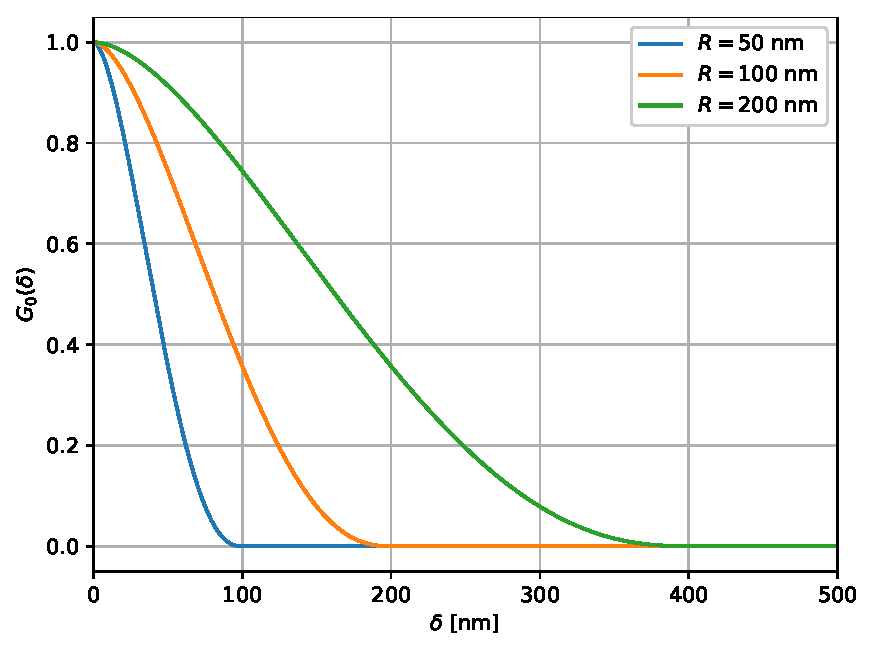
\includegraphics[width=0.5\linewidth]{analytical-G0}
	\caption{Normalized SESANS correlation function $G_0(\delta)$ curves for three dilute mono-disperse solid sphere samples with different radii $R$. The corresponding analytical expression is given by Equation \eqref{eq:sample-G0}.}
	\label{fig:analytical-G0}
\end{figure}

\newpage

\subsubsection{Solid sphere form factor and $Q$-range}
Formulated in terms of $Q$ as in regular SANS rather than $\delta$, the relevant $Q$-range of a dilute mono-disperse sample of spheres with radius $R$ can be seen to be largely determined by its form factor $P(Q)$ as $d\sigma(\vec{Q})d\Omega\propto P(Q)$, which is \cite{rekveldt1996}
\begin{equation}
	P(Q) = \left(3\frac{\sin(QR) - QR\cos(QR)}{\left(QR\right)^3}\right)^2\label{eq:sample-form-factor}
\end{equation}
This is a rapidly decaying oscillation with significant values in the range from $Q_{\text{min}} = 0.1/R$ up to $Q_{\text{max}} = 10/R$, meaning that in order to determine $G(\delta)$ accurately a detector should integrate over a proportional $Q$-range.  Figure \ref{fig:analytical-P} shows $P(Q)$ with these limits for $R = 100\unit{\nano\meter}$.  

\begin{figure}
	\centering
	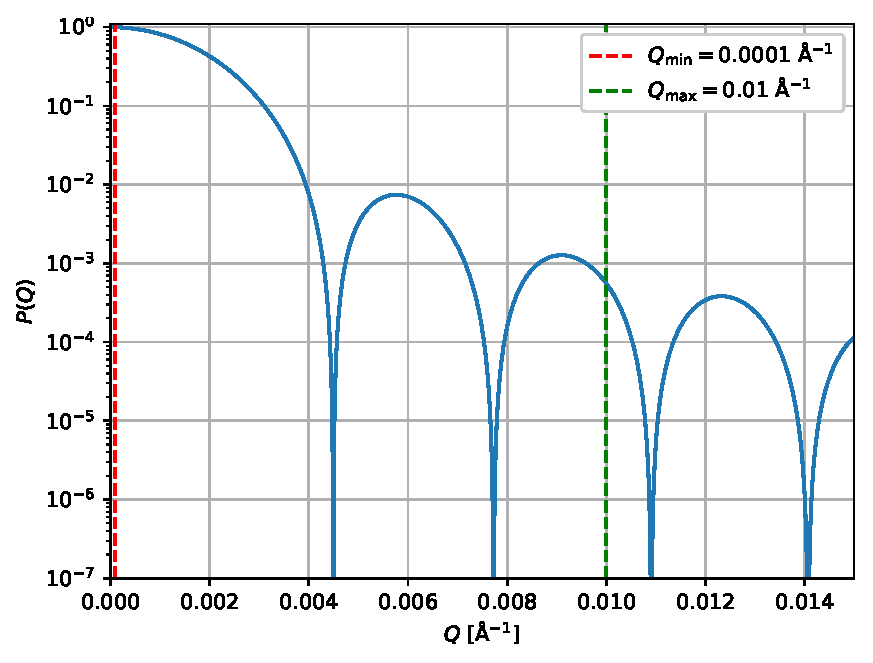
\includegraphics[width=0.5\linewidth]{analytical-P-log}
	\caption{Solid sphere form factor $P(Q)$ for $R = 100\unit{\nano\meter}$ with $Q_{min}, Q_{max}$ as given by Equation \eqref{eq:sample-form-factor}. It can be seen that for $Q > Q_{max}$, $P(Q) < 10^{-3}$ with its oscillation peaks decreasing in amplitude.}
	\label{fig:analytical-P}
\end{figure}

\newpage
\begin{figure}[hbtp]
	\centering
	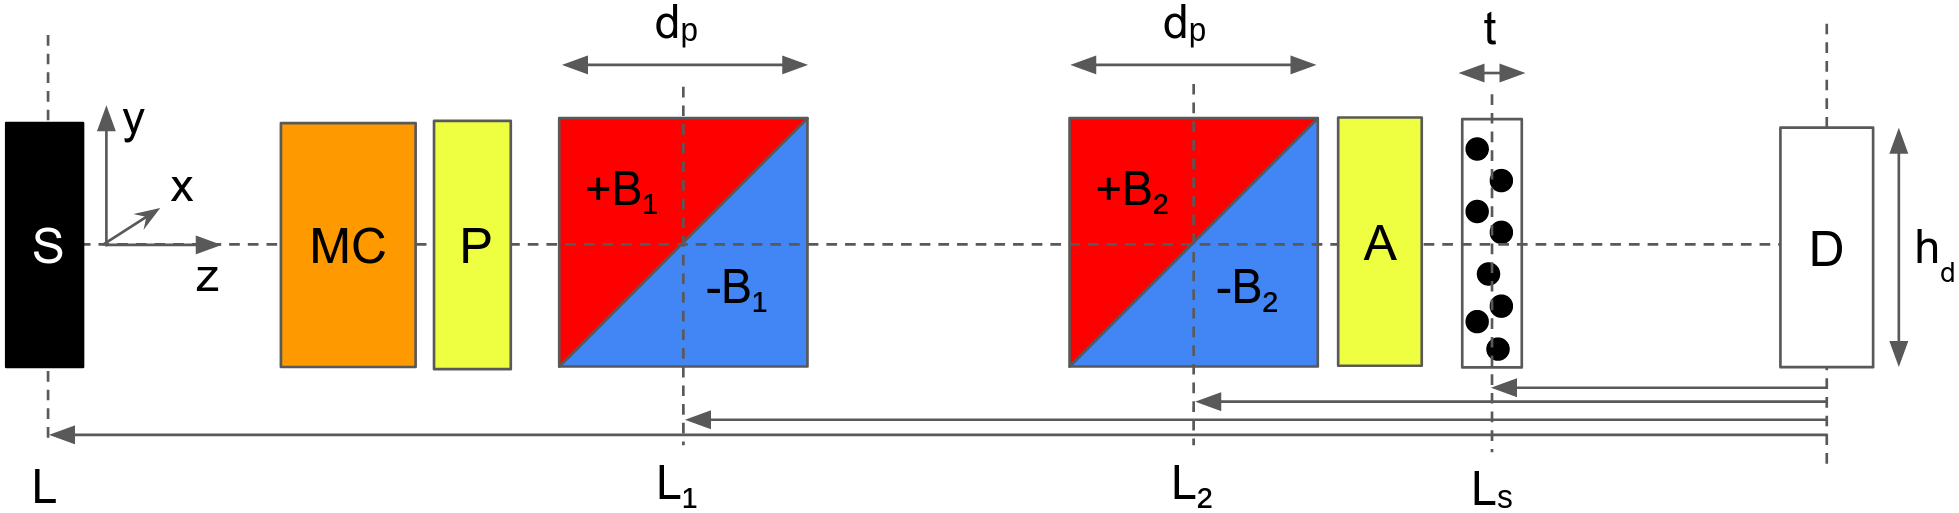
\includegraphics[width=\linewidth]{instrument-configuration}
	\caption{Schematic of the SEMSANS instrument configuration considered in this chapter, lengths and dimensions are not to scale. Neutrons are emitted from the source (S) after which they pass through a monochromator (MC) and are polarized in the $+x$ direction by a polarizer (P). The polarized neutrons travel through two precession devices (shown is a Wollaston prism as discussed in Section \ref{c3.3}) at distances $L_1, L_2$ from the detector and have field strength $\pm B_1$ and $\pm B_2$ in different field regions to create a $y$-dependence in the precession angle as discussed in Section \ref{c2.2}. The devices have depth $d_p$, which is also the approximate length travelled by neutrons through them. Next, the analyser (A) creates a modulated intensity pattern which scatters of the sample at distance $L_s$ with thickness $t$. This scattered intensity pattern arrives at the detector (D) with height $h_d$. The sample can be omitted to measure the unscattered modulation pattern, making it possible to compute the decrease in modulation amplitude related to $G(\delta)$ as per Equation \eqref{eq:sample-pol-reduction}.}
	\label{fig:instrument-config}
\end{figure}

\section{Instrument analysis for a cold source}
\label{c3}
In this chapter, the used SEMSANS instrument model is introduced and analysed. The cold neutron source and the applicable monochromators for different $\lambda_0$ ranges will be described and three different precession device options and their properties will be described. Additionally, the effect of a spread in wavelength $\lambda$ is described in terms of the observed modulation pattern as well as what is effectively measured. This is to account especially for the greater wavelength spread $\Delta\lambda/\lambda_0$ as encountered at higher $\lambda_0$ operating points accessible at a cold source, requiring the use of a velocity selector monochromator. In the last section, a list of instrument design variants considered in this research is introduced. These will be analysed and simulated in Chapter \ref{c4:constraints} and Chapter \ref{c6:monte-carlo} respectively. 

\subsection{Instrument configuration}
\label{c3.1}
The general configuration of the family of SEMSANS instruments considered in this work is illustrated in Figure \ref{fig:instrument-config}. It is derivative of an existing study simulating a SEMSANS instrument using foil-flippers and the corresponding McStas instrument \texttt{SEMSANS\_Delft} \cite{bouwman2021b}. Neutrons enter the instrument from a beamline, after which they pass through a monochromator set to select neutrons with a wavelength around $\lambda_0$, with  $\Delta\lambda/\lambda_0$ depending on the choice of monochromator as described below. Next, they pass through a polarizer and two precession devices at locations $L_1, L_2$ respectively. As described in Chapter \ref{c2:theory}, a modulated neutron intensity pattern appears after the analyser, which scatters of the sample at distance $L_s$ from the position-sensitive detector at the end, causing different degrees of loss of visibility of the modulation pattern depending on the sample structure as discussed in Section \ref{c2.3}. 

\subsection{Source beam characteristics and monochromators}
\label{c3.2}
The cold source beamline is assumed to have a spectrum corresponding to a Maxwell-Boltzmann distribution at $T = 20 \unit{\kelvin}$ given by 
\begin{equation}
	f_\lambda(\lambda) = \sqrt{\frac{2}{\pi}}\left(\frac{1}{mk_BT}\right)^{\frac{3}{2}}\frac{h^3}{\lambda^4}e^{-\frac{h^2}{2k_BTm\lambda^2}} \label{eq:cold-source-spectrum}
\end{equation}
This distribution is shown in Figure \ref{fig:source-spectrum}, with the thermal distribution at $T=290 \unit{\kelvin}$ also shown for reference. For simplicity, a uniform rectangular beam of size $10\times10\unit{\milli\meter}$ is used to model the beam and it is focussed on the middle $10\times10\unit{\milli\meter}$ of the detector. Each neutron originating from point $(b_x,b_y)$ in the beam will be aimed at a uniformly sampled random point $(d_x, d_y)$ on the detector, so assuming a distance $L = 5\unit\meter$ from beamline to detector the divergence will be at most $\psi_0 = 2\unit{\milli\radian}$ along the $x$ or $y$ axis and about $\psi_0 = 2.8\unit{\milli\radian}$ in total. This model corresponds to a rectangular setting of the \texttt{Source\_simple} McStas source component which will be used in Monte Carlo simulations in Chapter \ref{c6:monte-carlo}.  

% The peak for $T=20 \unit{\kelvin}$ corresponds to $E = k_bT = 1.7 \unit{\milli\electronvolt}$ as opposed to $E = 25.0 \unit{\milli\electronvolt}$ for thermal neutrons. 
\subsubsection{Monochromators}
A monochromator is used to select a narrow band of wavelengths around a central wavelength $\lambda_0$. In a practical instrument, a pyroletic graphite (PG) crystal monochromator can be used to do this up to roughly $\lambda_0 \approx 4.5 $Å. For greater wavelengths, a helical velocity selector (VS) can be used to select neutrons travelling at the right velocity. This is a mechanical device rotating at a great speed, and a lower practical limit of $\lambda_0 \approx 7$Å is used as lower $\lambda_0$ would require a too great RPM. Both types of monochromator are characterized by $\Delta\lambda/\lambda_0$, the ratio of the full-width-half-maximum (FWHM) of wavelengths $\Delta\lambda$ passed through and $\lambda_0$. In PG crystals, this is a function of the mosaicity of the crystal \cite{shapiro1972} and for VS monochromators it depends on the ratio of the angular aperture of slits and the pitch angle \cite{szewc2010}. This ratio is taken to be $\Delta\lambda/\lambda_0 = 0.01$ and $\Delta\lambda/\lambda_0 = 0.1$ for PG and VS monochromators respectively, roughly corresponding to the characteristics of components available for an eventual realization. In both analysis and simulations, the transfer of monochromators is taken to be a Gaussian centered at $\lambda_0$ with $\sigma = \frac{1}{2\sqrt{2\ln 2}}\Delta\lambda$. So in practice, the following Gaussian distribution will be used as a source spectrum in both analysis and simulations.
\begin{equation}
	f_\text{gauss}(\lambda) = \frac{1}{\sigma\sqrt{2\pi}} e^{-\frac{1}{2}(\frac{\lambda - \lambda_0}{\sigma})^2} \label{eq:gauss-spectrum}
\end{equation}
\begin{figure}
	\centering
	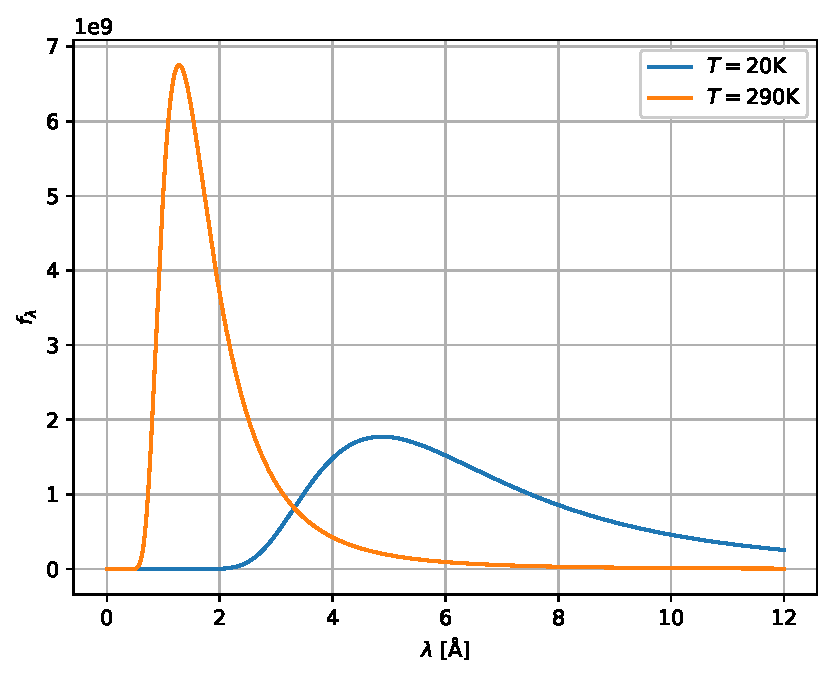
\includegraphics[width=0.5\linewidth]{source-spectrum}
	\caption{Probability density function for Maxwell-Boltzmann neutron sources at $T = 20 \unit{\kelvin}$ and $T = 290 \unit{\kelvin}$, illustrating the spectral differences. }
	\label{fig:source-spectrum}
\end{figure}
%% TODO: Discuss collimation, how the source in simulations will be focussed on the detector in a certain way etc. This lends itself to the language of collimation, divergence etc.
\subsection{Precession device analysis}
\label{c3.3}
As discussed in Chapter \ref{c2:theory}, different precession devices can be derived that give a precession angle of the form of Equation \eqref{eq:precession-freq} resulting in modulation. The three main types existent in literature are isosceles triangles \cite{sales2015}, magnetic Wollaston prisms \cite{li2021} and ferromagnetic foil flippers \cite{bouwman2021b} and all three have previously been used in SEMSANS realizations and simulations. Their respective geometries are shown in Figure \ref{fig:precession-devices}. What they all have in common is that their effect is proportional to $\cot(\theta)$ and magnetic field strength $B$.
\subsubsection{Isosceles triangles}
In the case of a triangle as illustrated in Figure \ref{fig:precession-devices:iso}, the angle of the faces with the $z$-axis can be seen to be $\theta_0 = \arctan\left(\frac{h}{d/2}\right)$. Consider the triangle to be centred along the optical axis so that $y=0$ bisects it. Then for a path at height $y$, the length $L$ passed through the field becomes
$$L = d/2 - \frac{2y}{\tan\theta_0}$$
Using the Equation \eqref{eq:larmor-prec}, the precession angle after passing through the triangle becomes
$$\phi = c\lambda B L = c\lambda B(d/2 - \frac{2y}{\tan\theta_0})$$
Next, consider two similar triangles with base $d_1, d_2$ and field strengths $B_1, B_2$. Adding their precession angles gives 
$$\phi = c\lambda (B_1d_1/2 +B_2d_2/2) - 2c\lambda (B_1 + B_2) \frac{y}{\tan\theta_0}$$
To achieve $\phi = 0$ at $y=0$, the condition $B_1d_1 = -B_2d_2$ must hold, giving 
$$\phi = -2c\lambda (B_1 + B_2) \frac{y}{\tan\theta_0}$$
This can be achieved by making the triangle with the stronger field the smallest. 

\subsubsection{Magnetic Wollaston prisms}
A more sophisticated device is the magnetic Wollaston prism shown in Figure \ref{fig:precession-devices:wsp}, having two equal and opposite triangular magnetic fields in the form of a square. The analysis is very similar to that of isosceles triangles and for a single prism with angle $\theta_0$, the precession angle is
$$\phi = \frac{2c\lambda B y}{\tan{\theta_0}}$$
Two prisms with fields $B_1, B_2$ in sequence gives
$$\phi = \frac{2c\lambda (B_1 + B_2) y}{\tan{\theta_0}}$$
\subsubsection{Ferromagnetic foil flippers}
The last device type considered is the ferromagnetic foil flipper depicted in Figure \ref{fig:precession-devices:foil}. It consists of a ferromagnetic foil of thickness $d = 3\unit{\micro\meter}$ in an electromagnet which quickly saturates to a magnetization of $B_s = 1.0 \unit{\tesla}$ \cite{kraan2003}. The foil has the effect of rotating neutron spins around it by an angle 
$$\phi_{foil} = \frac{cdB_s\lambda}{\sin\theta_0}$$
By appropriately choosing $\theta_0$, the foil can be made to rotate a central wavelength $\lambda_0$ by $\phi_{foil} = \pi$, causing the device to emulate a magnetic Wollaston prism using a simpler magnetic field as the effect of the second triangular region behind the foil will be opposite to that of the first for $\lambda = \lambda_0$. In this case,
$$\phi = -2c\lambda (B_1 + B_2) \frac{y}{\tan\theta_0}$$
For $\lambda \neq \lambda_0$ this will cause a depolarization as was previously shown experimentally \cite{kraan2003}.
% I think because there is then a y-component of spin which shows up as 50/50 up/down on the detector. 
\begin{figure}[htbp]
	\centering
	\begin{subfigure}[b]{0.3\textwidth}
		\centering
		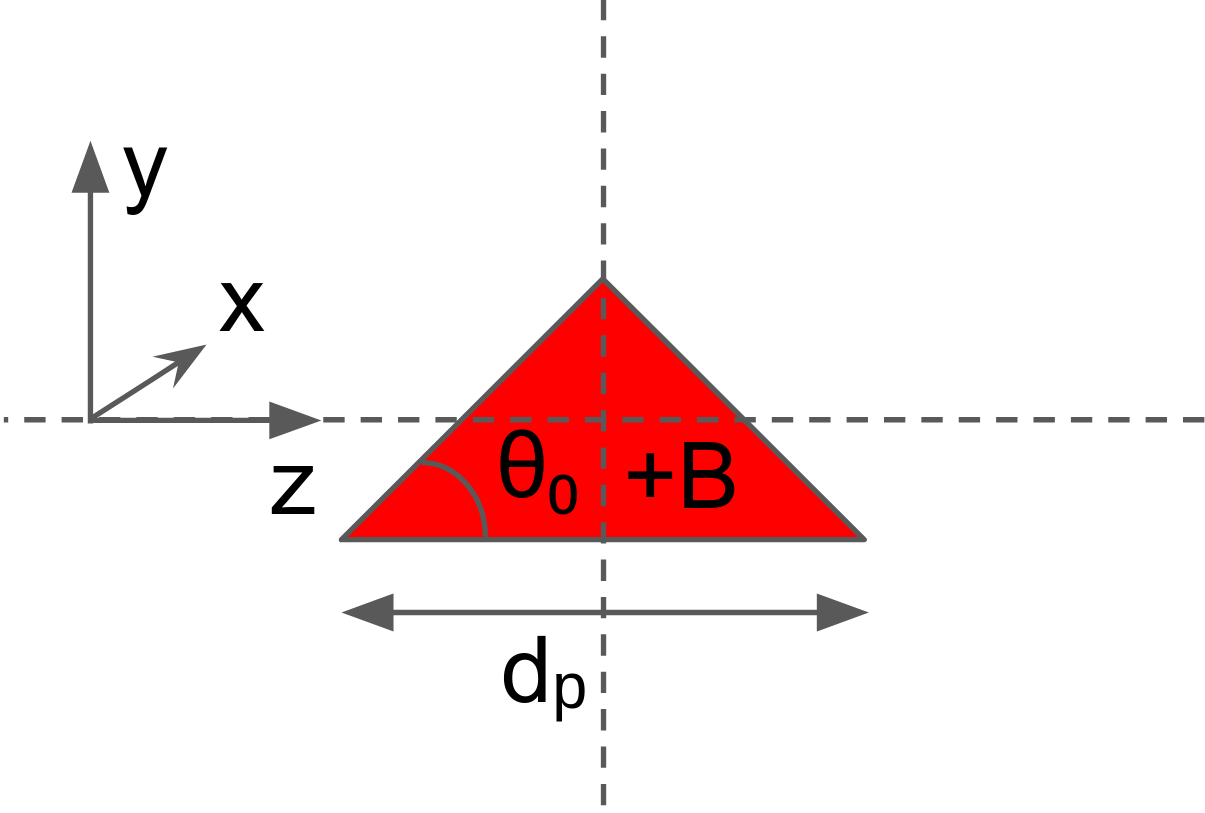
\includegraphics[width=\textwidth]{iso-schematic}
		\caption{Isosceles triangle}
		\label{fig:precession-devices:iso}
	\end{subfigure}
	\hfill
	\begin{subfigure}[b]{0.3\textwidth}
		\centering
		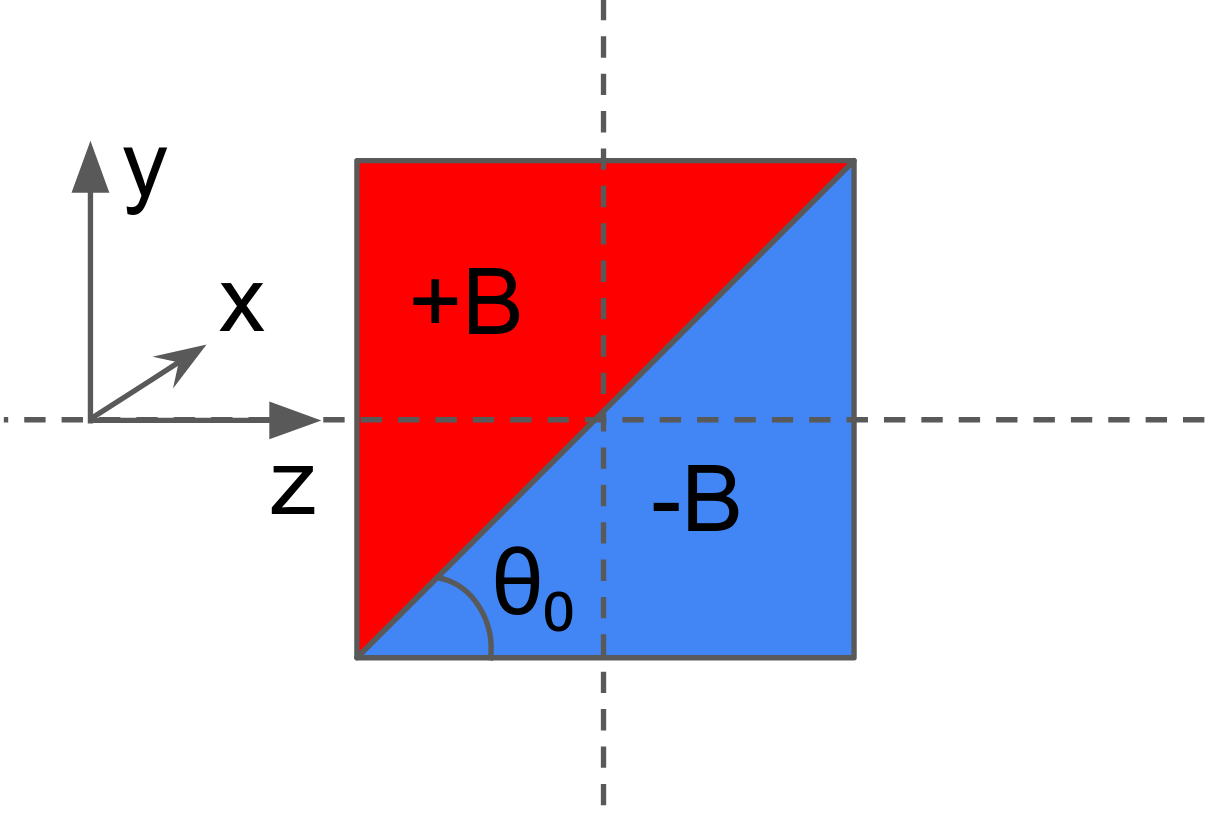
\includegraphics[width=\textwidth]{wp-schematic}
		\caption{Magnetic Wollaston prism}
		\label{fig:precession-devices:wsp}
	\end{subfigure}
	\hfill
	\begin{subfigure}[b]{0.3\textwidth}
		\centering
		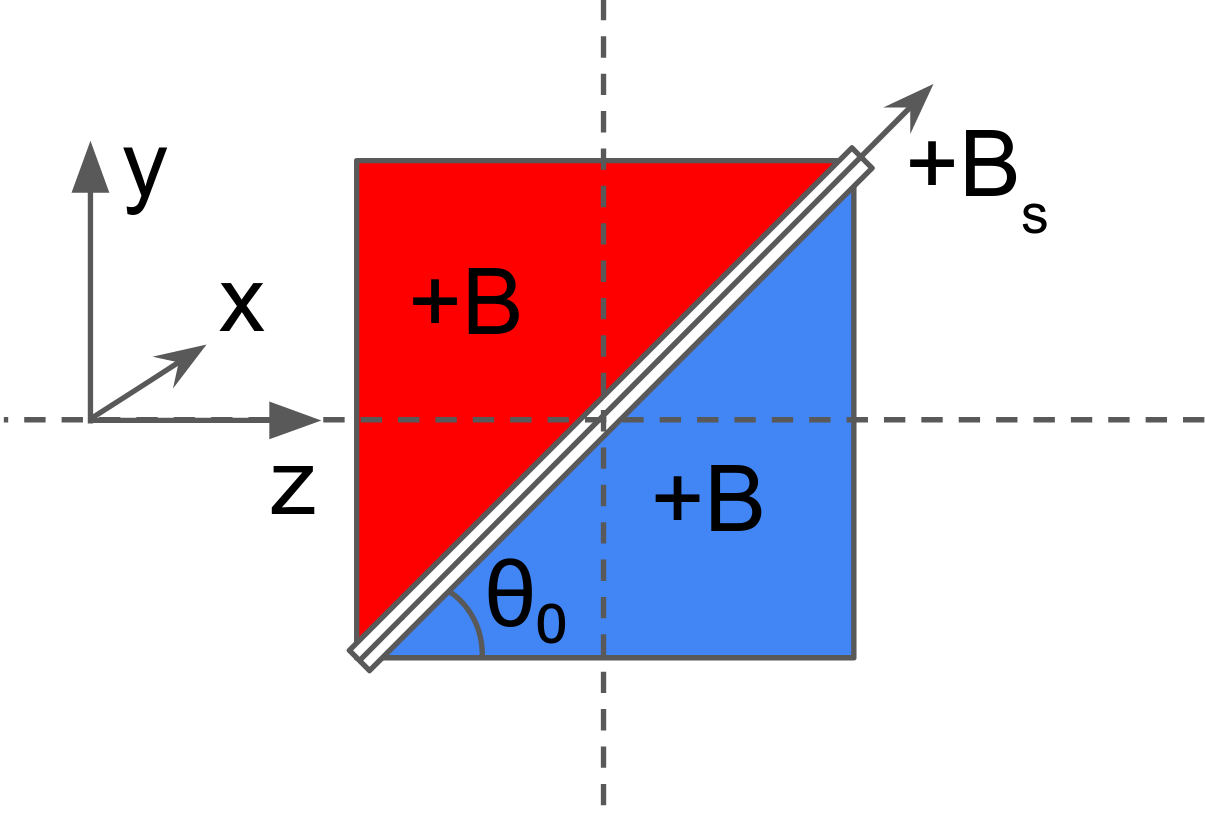
\includegraphics[width=\textwidth]{foil-schematic}
		\caption{Ferromagnetic foil flipper}
		\label{fig:precession-devices:foil}
	\end{subfigure}
	\caption{Schematics for the three different types of precession devices. Assuming positive $B$, the red areas represent a magnetic field in the $+y$ direction and blue areas a field in the $-y$ direction, with exception of Figure \ref{fig:precession-devices:foil}. The reason for this is that the field inside the ferromagnetic foil effectively flips the precession of neutrons of the right $\lambda_0$, causing the positive field after the foil to have the effect of a negative field, simulating the fields seen in a Wollaston prism as shown in Figure \ref{fig:precession-devices:wsp}. For all precession devices the field interfaces are canted by $\theta_0$ in the $yz$-plane and all have depth $d_p = 0.3\unit\meter$ as indicated in Subsection \ref{c3.3.4}. Only for Wollaston prisms $\theta_0 = 45 ^\circ$ as shown, with isosceles triangles in practice having $\theta_0 = 20^\circ$ and $\theta_0$ being a function of $\lambda_0$ in the case of foil flippers.}
	\label{fig:precession-devices}
\end{figure}

\subsubsection{Device $\alpha$ and characteristics}
\label{c3.3.4}
To summarize the above discussion of the three available devices, once device-specific conditions are met a pair of any of them have in absolute terms the same precession-angle profile given by Equation \eqref{eq:precession-freq} with $\alpha = \frac{(B_1 + B_2)}{\pi\tan\theta_0}$
\begin{equation}
	\phi = 2c\lambda (B_1 + B_2)\frac{y}{\tan\theta_0} \label{eq:device-prec}
\end{equation}
the contribution of each separate device being $\phi_i = \frac{2c\lambda B_i y}{\tan\theta_0}$. $\theta_0$ is a function of $\lambda_0$ for foil flippers and is fixed for Wollaston prisms and isosceles triangles, meaning that $B_1, B_2$ will in practice be set to vary $\alpha$. Table \ref{tab:device-properties} summarizes device characteristics as they appear in literature that will be used in this research. All devices are assumed to have depth $d_p = 0.3 \unit{\meter}$, limiting possible values of $L_1, L_2$ and $L_s$. 

\begin{table}[h!]
	\centering
	\begin{tabular}{|c|c|c|c|c|c|}
		\hline
		Name & Label & $\theta_0$ (degrees) & $B_{\text{min}}$ (mT) & $B_{\text{max}}$ (mT) & Source \\
		\hline
		Isosceles triangle & ISO & 20 & 0.1 & 15 & \cite{kusmin2017} \\
		Wollaston prism & WSP & 45 & 0.1 & 63 & \cite{li2021} \\
		Foil flipper & FOIL & - & 0.3 & 30 & \cite{bouwman2011} \\
		\hline
	\end{tabular}
	\caption{Precession device characteristics including the source of the values used. For a foil flipper, $\theta_0$ needs to be set to match $\lambda_0$ and is omitted, its range is sufficient for all $\lambda_0$'s considered in this research.}
	\label{tab:device-properties}
\end{table}
\subsubsection{Focussing condition}
In practice, neutrons will not travel parallel to the $z$-axis but move at a slight angle to this depending on beam divergence and other parameters. Letting $\psi$ be the angle their trajectory makes with the $z$-axis in the $yz$ plane, it can be seen that a neutron arriving at height $y$ on the detector will pass through the $i$'th precession device at average height $y_i = y + L_i\tan\psi \approx y + L_i\psi$, with $L_i$ being the distance from the detector of the device. This means that the total precession angle will be
$$\phi = 2c\lambda B_1\frac{y + L_1\psi}{\tan\theta_0} + 2c\lambda B_2\frac{y + L_2\psi}{\tan\theta_0}$$
This $\psi$-dependence is a problem as it will cause a loss of modulation depending on how large the variation in $\psi$ is. In first-order approximation, this effect can be removed by setting the positions $L_i$ and field strengths $B_i$ to meet the focussing condition
$$B_1L_1 = -B_2L_2$$
Substituting this retrieves Equation \eqref{eq:device-prec}. This gives also the motivation for using two devices: you need at least two to remove this $\psi$-dependency and achieve optimal modulation using a realistic, slightly divergent beam such as the one described above with $\psi_0 = 2\unit{\milli\radian}$.
\subsection{Detector characteristics and $Q$-range}
\label{c3.4}
The position sensitive detector used is $11\times11\unit{\milli\meter}$ with a resolution of $1001$ pixels along the $y$-axis, corresponding to a pixel size of approximately $p = 10.98\unit{\micro\meter}$ with detector height $h_d = 11\unit{\milli\meter}$. As will be discussed in Chapter \ref{c4:constraints}, $h_d$ and $p$ limit the modulation frequencies $f = \alpha\lambda$ that can be sampled. The detector is placed at distance $L_s$ from the sample, meaning that ignoring divergence and assuming a straight beam, scattering from point $s_y = 0$ on the sample will be limited to angle $\theta_a = h_d/(2L_s)$ in small-angle approximation, resulting in a maximum wave-vector transfer of $Q_\text{max} \approx \frac{2\pi}{\lambda_0}\theta_a$. A fuller discussion of which angles are accepted by each point $y$ on the detector depending on beam collimation, sample size and detector characteristics is given in \cite{kusmin2017}. Generally speaking, it can be seen that a detector can be used to integrate an experimental estimate $G_\text{exp}(\delta)$ of $G(\delta)$ as given in Equation \eqref{eq:G-analytical} limited by such a $Q_\text{max}$, given by 
\begin{equation}
	G_\text{exp}(\delta) = \frac{t}{k_0^2}\int_{-Q_\text{max}}^{Q_\text{max}}\int_{-Q_\text{max}}^{Q_\text{max}}\dfrac{d\sigma(\vec{Q})}{d\Omega}\cos(Q_y \delta)dQ_xdQ_y  \label{eq:G-experimental}
\end{equation}
assuming a symmetric detector with an equal $Q$-range for $x,y$. For samples with significant scattering with $Q > Q_{max}$, the error of $G_\text{exp}(\delta)$ as estimator of $G(\delta)$ can be expected to be significant whereas for samples with larger characteristic lengths and scattering over lower $Q$-ranges, the error will be negligible with most scattered neutrons being picked up by the detector \cite{rekveldt1996} so that $G_\text{exp}(\delta)$ approximates $G(\delta)$ well. 

\subsection{The sample and its position $L_s$}
\label{c3.5}
The model sample that is considered in this work is a dilute mono-disperse solution of solid spheres as described in Section \ref{c2.4} with radii varying from $R = 50\unit{\nano\meter}$ to $R = 2000\unit{\nano\meter}$. It is modelled as a $20\times20\unit{\milli\meter}$ square with thickness $t$ along the $z$-axis, meaning that it is significantly wider than the beam as described above. 
 
In general, $L_s$ can be varied in a given instrument to measure different samples in practical SEMSANS instrument designs \cite{kusmin2017}. However, as mentioned in Section \ref{c1.2}, one of the target applications of the instrument is to study processes in colloids like milk turning into yoghurt which encompass the full target range of $10 \unit{\nano\meter}$ to $5 \unit{\micro\meter}$. This means that it is not practical to adjust $L_s$ in the middle of measurements as it would require precise remote control of the sample holder. It is assumed that such control is not available in this model and that for a given sample measurement $L_s$ is fixed, although measurements can be performed at different $L_s$.  

\subsubsection{Permissible sample positions $L_s$}
When placing a sample in a given instrument, an important criterion is that $h_d/L_s$ needs to be small enough so that the small-angle approximation $Q_{max} \approx \frac{2\pi}{\lambda_0}\frac{h_d}{2L_s}$ remains valid. As derived in Appendix \ref{appendix-a}, a third-order approximation of $Q_{max}$ is given by
$$Q_{max} \approx  k(\frac{h_d}{2L_s} - \frac{3h_d^3}{64L_s^3})$$
making the relative approximation error proportional to $\epsilon_\angle = \frac{3h_d^2}{32L_s^2}$. What values of $h_d/L_s$ and $\epsilon_\angle$ are permissible is unclear as no studies appear to have been done investigating this specifically. Values like $\theta_a \approx 30\unit{\milli\radian}$ are used in SESANS \cite{rekveldt1996} however, indicating that a tenfold increase might be feasible although it is not obvious if this can be translated to a SEMSANS acceptance angle. To be on the safe side, $\theta_a = \arctan\left(h_d / (2L_s)\right) = 15\unit{\milli\radian}$ will be used as an upper limit in this work, translating to a lower limit of $L_{s,min} = 0.366\unit{\meter}$ for $h_d = 11\unit{\milli\meter}$. 
The upper limit of $L_s$ is determined by the depth of the second precession device $d_p$, its position $L_2$ and sample thickness $t$, giving $L_{s,max} = L_2 - d_p / 2 - t/2$, which evaluates to $L_{s,max} = 1.845 \approx 1.8\unit\meter$ for $L_s$ and assuming maximum sample depth $t=0.01\unit\meter$. Analyser and sample holder dimensions will in practice further limit $L_s$ but this is ignored in this simple model.

%% TODO: add min Q from pixel size? I guess in small angle approximation this is already in there? In fact probably Q_max will already be related to the period although I need to figure out how exactly. 
\subsection{Polychromatic SEMSANS}
\label{c3.6}
The usual description of SEMSANS modulation patterns as given in \eqref{eq:mono-modulation} and their relation to a spin-echo length \eqref{eq:delta} typically assumes a monochromatic source or a source that closely approximates it, for instance by using a PG monochromator with $\Delta\lambda/\lambda_0 = 0.01$ with thermal neutrons. However, even in such cases a modulation envelope can be seen to appear \cite{bouwman2021} due to this wavelength spread. This effect becomes far more important when using a velocity selector with $\Delta\lambda/\lambda_0 = 0.1$ to select a higher wavelength $\lambda_0$ and is here discussed in detail.
%Without resorting to time-of-flight instrument realizations also exist \cite{sales2015}\cite{li2021} that in this way support broad ranges of wavelengths. 
\subsubsection{Modulation envelope for Gaussian $\lambda$ spectrum}
Assuming a Gaussian wavelength distribution as given by Equation \eqref{eq:gauss-spectrum} and neglecting wavelength-specific effects like foil flipper polarization loss, it can be shown using Fourier analysis that the base intensity modulation becomes
\begin{equation}
	I_b(y) = I_{0,b} \pm A_bE(y)\cos(2\pi\alpha\lambda_0y) \label{eq:poly-base-modulation}
\end{equation}
The envelope $E(y)$ is a Gaussian and given by
\begin{equation}
	E(y) = e^{-\frac{1}{2}\left(2\pi\alpha\sigma y\right)^2} \label{eq:poly-base-modulation-env}
\end{equation}
Substituting $\sigma=0$ for a monochromatic limit gives back Equation \eqref{eq:mono-modulation}. This modulation envelope $E(y)$ can be shown to have FWHM 
\begin{equation}
	FWHM_E = \frac{\sqrt{2\ln 2}}{\pi\alpha\sigma} \label{eq:poly-base-modulation-fwhm}
\end{equation}
From this it can clearly be seen that increasing wavelength spread $\sigma$ results in a narrower modulation envelope width. It also confirms the envelope narrowing observed when increasing $B$ field strengths (proportional to $\alpha$) \cite{bouwman2021}. 
\subsubsection{Effect on interaction with sample and $\delta$-resolution}
At first glance, it is clear that the effect of a sample on the modulation will be more complicated than a simple reduction of the amplitude of the modulation envelope. The modulation now consists of a range of wavelengths $\lambda$, each related to a spin-echo length $\delta = \lambda^2 L_s\alpha$ and each with a scattering power $\tau \propto\lambda^2$ such as Equation \eqref{eq:sample-tau}. Although Equations \eqref{eq:mono-modulation} and \eqref{eq:sample-pol-reduction} by itself do not describe the corresponding modulation pattern, they do describe what happens to a single frequency so that
\begin{equation}
	I_s(y) = I_{0,s} + \int_{-\infty}^\infty f_{\text{gauss}}(\lambda)e^{G(\lambda^2 L_s\alpha) - \tau(\lambda)}A_b\cos(2\pi\alpha\lambda y)d\lambda \label{eq:poly-sample-modulation}
\end{equation}
per linearity describes the modulation pattern. Qualitatively it can be seen that for greater $\sigma$, a greater $\delta$ range is accessed around a central value corresponding to $\lambda_0$ and reflected in the spectrum. This means that estimating $G(\delta)$ from the visibility will introduce error depending on the specific sample and the $\delta$-resolution will be limited. One way to avoid this problem is to compute the Fourier spectrum and consider the transfer of the sample in the frequency domain. This does bring with it new problems such as frequency resolution limitations. 


\subsection{Instrument design variants}
\label{c3.7}
Using the basic instrument configuration described and analysed in this chapter with the various options in terms of monochromator and precession devices, a few design variants can be formulated exploring the different options for these component types. Firstly, there is the choice of $\lambda_0$ and the corresponding monochromator. Two considered options are $\lambda_0 = 4.321$Å with a PG monochromator giving $\Delta\lambda = 0.04321$Å and $\lambda_0 = 8$Å with a VS monochromator giving $\Delta\lambda = 0.8$Å. These two sources are combined with each of the three precession device options as characterized in Table \ref{tab:device-properties}, giving Table \ref{tab:design-variants} which includes the appropriate $\theta_0$ needed to achieve $\phi_{foil} = \pi$ in the case of foil flippers. These instruments will first be analysed in the next chapter to estimate their $\delta$-range by using constraints as well as their relative source intensity. In Chapter \ref{c6:monte-carlo}, Monte Carlo simulation results of these instruments on a three representative samples are discussed. 

What the designs have in common are the precession device positions $L_1 = 4.0\unit{\meter}, L_2 = 2.0\unit{\meter}$. Additionally, the detector dimensions are $11\times 11\unit{\milli\meter}$ with pixel size $p = 10.98 \unit{\micro\meter}$ and a distance from source to detector of $d = 5\unit\meter$, summarizing from what is given above. For simplicity and to facilitate comparison, the approximate maximum value of $L_s = 1.8\unit{\meter}$ will be used in all calculations for the designs, including the computed constraints in Chapter \ref{c4:constraints} and the Monte Carlo simulations presented in Chapter \ref{c6:monte-carlo}. The possibility of optimizing distances $L_1, L_2, L_s$ together with $\lambda_0$ for a given choice of monochromator and precession device is discussed in Chapter \ref{c5:optimization}.  


\begin{table}[h!]
	\centering
	\begin{tabular}{|c|c|c|c|c|c|c|c|}
		\hline
		Label & $\lambda_0$ (Å) & $\Delta\lambda$ (Å) & Monochrom. & Device & $\theta_0$ (degrees) & $B_{\text{min}}$ (mT) & $B_{\text{max}}$ (mT) \\
		\hline
		ISO 4.321 & 4.321 & 0.04321 & PG & ISO & 20 & 0.1 & 15 \\
		WSP 4.321 & 4.321 & 0.04321 & PG & WSP & 45 & 0.1 & 63 \\
		FOIL 4.321 & 4.321 & 0.04321 & PG & FOIL & 11.013 & 0.3 & 30 \\
		ISO 8 & 8 & 0.8 & VS & ISO & 20 & 0.1 & 15 \\
		WSP 8 & 8 & 0.8 & VS & WSP & 45 & 0.1 & 63 \\
		FOIL 8 & 8 & 0.8 & VS & FOIL & 20.714 & 0.3 & 30 \\
		\hline
	\end{tabular}
	\caption{Various instrument design variants combining different $\lambda_0$ and monochromator pairings with the various precession device options. Designs are labelled by combining their device type and the value of $\lambda_0$ in Å.}
	\label{tab:design-variants}
\end{table}

% $\psi_0 = 1^\circ$ or $\psi_0 = 0.01745329$ in radians



%\section{SEMSANS instrument model}
%In this chapter, the used SEMSANS instrument model and all its components with their basic functions as well as parameters is introduced. It is based on an instrument which was previously simulated (CITATION NEEDED) and which is available as NAME in the McStas instrument library. A schematic overview is given in ADD FIGURE HERE. 
%\subsection{Source}

%\section{Source}
% Key challenge: translate this beautiful blob of mathematics and analysis I have in my jupyter notebook to on the one hand a summary and theoretical background and on the other hand a (somewhat, at least in the extent of having fully worked it out myself generally unaware of existing derivations) novel analysis on which
% Another challenge: how to deal with the rather expansive theory with at least 2 main branches which there appears to be? If I give a theoretical background to make this thing readable for other bachelor students then I do sort of have to start at Larmor precession and neutron spins but also at small angle scattering and this is confusing. 

\newpage
\section{$\delta$-constraints and intensity in instrument design}
\label{c4:constraints}
Two key parameters in SEMSANS instrument design are the accessible $\delta$-range and the intensity at the detector. The first determines the range of samples that can be measured and the second the amount of signal per unit time, which determines how well you can measure in given time or similarly the measurement time needed for a required measurement quality. In this chapter, building on the analysis presented in Chapter \ref{c3}, a system of constraints will be presented that together limit the accessible $\delta$ range for each of the designs listed in Table \ref{tab:design-variants}. After discussing the $\delta$-ranges, a coarse estimate for the intensity at the detector for the two source options will be presented. Lastly, the effect of intensity loss due to SANS scattering is discussed by using a very primitive model for scattering based on the sample form factor $P(Q)$, the goal being to understand the lower $\delta$-limit of the presented instruments better.
\subsection{Constraints}
\label{c4.1}
Three main sources of limitations can be recognized. Firstly, the detector height $h_d$ and pixel size $p$ as well as the distance from detector to sample $L_s$ will limit which modulation frequencies can be sampled as well as the accessible $Q$-range, limiting $\delta$ in various ways.
Secondly, the mean wavelength $\lambda_0$ as well as the monochromator quality $\frac{d\lambda}{\lambda_0}$ (and corresponding wavelength $\sigma$) shape the modulation envelope and determine how quickly it will become too narrow as $\alpha$ increases due to increasing field strengths, with $\lambda_0$ also playing a role in all other bounds. Lastly, the basic characteristics of precession devices as well as their positions relative to the detector limit the range of $\alpha$ and how strong the precession gradient is along the $y$-axis. 

% Discuss sources of constraints, linking them to the theory in previous chapters. Ideally refer to equation numbers to avoid repetition and make it sound really solid. 
% Emphasize that these constraints serve as a starting point for estimating limitations for given instruments
\subsubsection{Detector sampling limitations}
Using detector sampling frequency $f_s = \frac{1}{p}$, the Nyquist frequency is $f_n = f_s/2$ and this an exclusive upper-limit at two samples per modulation period, corresponding to 
$$\delta_{max,n} = \frac{\lambda_0L_s}{2p}$$
This can be derived from the form of $\delta$ that is independent of $\alpha$, $\delta = \lambda_0 fL_s$. In practice, modulation visibility is reduced when approaching this frequency. One way to reduce this is to set a bound for this effect and solve it numerically as done in \cite{kusmin2017}. A simple alternative to this is to require more samples per period, for instance $10$ instead of $2$ giving
$$\delta_{max,s} = \frac{\lambda_0L_s}{10p}$$
Similarly, the requirement that at least 1 modulation period is visible on the detector restricts the frequency to a minimum of $f_{min} = \frac{1}{h_d}$, corresponding to 
$$\delta_{min,s} = \frac{\lambda_0L_s}{h_d}$$
An alternative and equivalent way of deriving this is through considering the detected $Q$-range, using $Q_{max}$ and $\theta_a$ as described in Section \ref{c3.4}. This gives 
$$Q_{max} = \frac{\pi h_s}{\lambda_0 L_s}$$
This is equivalent to $\delta_{min,s}$ as it satisfies $\delta_{min,s} Q_{max} = \pi$. It also provides an idea of the $Q$-range that reaches the detector, providing a coarse upper limit for $Q$ and accessible characteristic sample lengths. 

\subsubsection{Modulation envelope width}
As discussed before, the modulation can be described by a Gaussian envelope with a FWHM as given by Equation \eqref{eq:poly-base-modulation-fwhm}. Using $\delta = \lambda_0^2L_s\alpha$ and given a $FWHM_{e,min}$, this can be rewritten to a maximum $\delta$ value
$$\delta_{max,e} = \frac{\sqrt{2\ln 2}\lambda_0^2 L_s}{\pi\sigma FWHM_{e,min}}$$
In this way, the intuitive notion that the envelope should not become too narrow to measure enough signal can be translated to a concrete limit by choosing $FWHM_{e,min}$. For monochromators with a low $\Delta\lambda$ and a corresponding low $\sigma$ such as PG monochromators, this will in practice not normally be a limit but it can be when using velocity selectors. The chosen value in this work for $FWHM_{e,min}$ is $2 \unit{\milli\meter}$, so about $18.2$\% of the detector height $h_d$ and is somewhat permissive.  

\subsubsection{Precession device limitations}
In terms of instrument design, the engineering of precession devices with a high $\alpha$ and optimizing their positions from the detector $L_1, L_2$ perhaps has the greatest impact on $\delta$-range. The importance of $L_1, L_2$ comes from the focussing condition, which is $B_1L_1 = -B_2L_2$ for two devices. As $\alpha\propto B_1 + B_2$ and $B_1, B_2$ are each limited by device-specific $B_{min}, B_{max}$ as given by Table \ref{tab:device-properties}, $B_1 + B_2$ is bounded by
$$(B_1 + B_2)_{min} = (\frac{L_1}{L_2} - 1)B_{min}$$
$$(B_1 + B_2)_{max} = (1 - \frac{L_2}{L_1})B_{max}$$
For the minimum value, $B_1 = B_{min}$ and for the maximum value, $B_2 = B_{max}$ with the other set accordingly. Using $\alpha = \frac{c(B_1+B_2)}{\pi\tan\theta_0}$, the following $\delta$ constraints can be derived
$$\delta_{min, f} = \lambda_0^2 L_s \frac{c(\frac{L_1}{L_2} - 1)B_{min}}{\pi\tan\theta_0}$$
$$\delta_{max, f} = \lambda_0^2 L_s \frac{c(1 - \frac{L_2}{L_1})B_{max}}{\pi\tan\theta_0}$$

\begin{table}[h!]
	\centering
	\begin{tabular}{c | c c | c c c}
		\toprule
		Label & $\delta_{\text{min,s}}$ (nm) & $\delta_{\text{min,d}}$ (nm) & $\delta_{\text{max,s}}$ (nm) & $\delta_{\text{max,e}}$ (nm) & $\delta_{\text{max,d}}$ (nm) \\
		\midrule
		FOIL 4.321 & 70.71 & \textbf{76.35} & 7077.8 & 34321.19 & \textbf{3817.27} \\
		WSP 4.321 & \textbf{70.71} & 4.95 & 7077.8 & 34321.19 & \textbf{1560.21} \\
		ISO 4.321 & \textbf{70.71} & 13.61 & 7077.8 & 34321.19 & \textbf{1020.63} \\
		FOIL 8 & 130.91 & \textbf{134.69} & 13104.0 & \textbf{6354.31} & 6734.57 \\
		WSP 8 & \textbf{130.91} & 16.98 & 13104.0 & 6354.31 & \textbf{5348.03} \\
		ISO 8 & \textbf{130.91} & 46.65 & 13104.0 & 6354.31 & \textbf{3498.48} \\
		\bottomrule
	\end{tabular}
	\caption{Calculated $\delta$ constraints for the designs with the constraints limiting the final $\delta$-range listed in Table \ref{tab:designs-final-ranges} marked in bold for each design.}
	\label{tab:designs-delta-constraints}
\end{table}
\subsection{Computed $\delta$ constraints and design $\delta$ ranges}
\label{c4.2}
The computed $\delta$-constraints for the designs are given in Table \ref{tab:designs-delta-constraints}. From these together, $\delta$-ranges can be calculated for each design as given in Table \ref{tab:designs-final-ranges} together with their $Q_{max}$. %These values were computed using $L_s = 1.8\unit\meter$, which is approximately the maximal $L_s$ setting available. This means that shorter $\delta_{min}$ is accessible by reducing $L_s$ but $\delta_{max}$ is the maximal spin-echo length that can be measured.
\begin{table}[h!]
	\centering
	\begin{tabular}{c c c c}
		\toprule
		Label & $Q_{\text{max}}$ ($\text{\AA}^{-1}$) & $\delta_{min}$ (nm) & $\delta_{max}$ (nm) \\
		\midrule
		FOIL 4.321 & 0.00444 & 76.35 & 3817.27 \\
		WSP 4.321 & 0.00444 & 70.71 & 1560.21 \\
		ISO 4.321 & 0.00444 & 70.71 & 1020.63 \\
		FOIL 8 & 0.0024 & 134.69 & 6354.31 \\
		WSP 8 & 0.0024 & 130.91 & 5348.03 \\
		ISO 8 & 0.0024 & 130.91 & 3498.48 \\
		\bottomrule
	\end{tabular}
	\caption{Key characteristics for the various designs, with $\delta_{min}, \delta_{max}$ being computed using the constraints listed in Table \ref{tab:designs-delta-constraints}}
	\label{tab:designs-final-ranges}
\end{table}
\subsubsection{Discussion of design constraints}
The computed $\delta$-ranges and $Q_{max}$ give a first understanding of for what samples the designs can be used to estimate $G(\delta)$ through $G_{\text{exp}}(\delta)$. $\delta$ limits the range of $G(\delta)$'s that can be estimated and $Q_{max}$ gives an indication of how well the bounded integral will approximate the true value. It can be seen that instruments at $\lambda_0 = 4.321$Å have a wider $Q$-range given the same $L_s, h_d$ as was to be expected from $Q_{max} \propto 1/\lambda_0$ and correspondingly a lower $\delta_{min}$, making them better able to characterize samples of $\delta \approx 100 \unit{\nano\meter}$. For instruments with triangles and prisms, the condition that at least one modulation period must fit on the detector of height $h_d$ is a limiting factor, whereas for foils the devices and their positions $L_1, L_2$ limit $\delta$. Another observation that can be made is that instruments at $\lambda_0 = 4.321$Å with a narrower $\lambda$ spectrum are limited more strongly by the upper sampling limit due to detector pixel size $p$ whereas with a wider spectrum at $\lambda_0 = 8$Å the narrowing of the modulation envelope becomes a limiting factor. With exception of FOIL 8, the upper $\delta$ limit is in these instruments determined by device characteristics together with $L_1, L_2, L_s$ as well as the specific $\lambda_0$ operating point. 


\subsubsection{Limitations of constraint scheme}
Together, the constraints above give an impression of various factors limiting the achievable $\delta$-range for SEMSANS instruments with $2$ precession devices. It makes it possible to quickly evaluate designs such as those given and identify possibilities to improve them by making the necessary changes. There are some key limitations however, in particular related to the beam and the detector $Q$-range. As mentioned in Section \ref{c3.4} it is assumed that the full detector height $h_d$ is covered by the beam which translates to requirements for the beam width and/or divergence. The intensity across the beam is assumed to be uniform, which means that the used Gaussian modulation pattern might be too simple of a model for the modulation envelope. As for the $Q$-range, the lower limit imposed by sampling and the precession devices might be too permissive as in practice at the smallest $\delta$, $Q_{max}$ can be too low and $G_\text{exp}(\delta)$ can significantly deviate from $G(\delta)$, this will be discussed in Section \ref{c4.4}. $B$-resolution limitations and how these could influence the $\delta$-resolution were also not considered. Lastly, all computed constraints are derived from values as listed in Table \ref{tab:device-properties} and elsewhere meaning that if say improved precession devices are available with greater $B_{max}$ or different $\theta_0$, the constraints need to be reevaluated.  
%Some factors that were not taken into account are errors in $G_\text{exp}$ for the lowest $\delta$ values where the $Q$-range might be insufficient as well as more acc

 
% Discuss things that are missing
%Also very important: discuss the softer constraints: why should the envelope FWHM be 3mm and not 2mm or 4mm? What determines this other than vibes. Indicate how they could be made more/less flexible		




\subsection{Intensity estimate}
\label{c4.3}
In this section, a coarse estimate of intensities as they can be expected using the described designs is derived. Although accurate intensity estimates are beyond the scope of this research, requiring detailed characterizations of losses in all components as well detailed information about the newly installed cold source, a highly simplified estimate assuming ideal components can be derived as follows.

The original targetted value for the full-spectrum flux at the new cold source beamline corresponding to a reactor power of $3\unit{\mega\watt}$ of $10^9 \unit{\centi\meter^{-2}\sec^{-1}}$ \cite{OYSTER2008} is taken as a starting point. It is assumed that the intensity of the source has about half the original targetted intensity, so $\Phi_0 = 5\cdot 10^8\unit{\centi\meter^{-2}\sec^{-1}}$. Given an operating point $\lambda_0$ with a matching $\sigma$ from the monochromator type, the intensity can be estimated by numerical evaluation of the integral
$$\Phi_{mc} \propto \int_0^\infty f_\lambda(\lambda)e^{-\frac{1}{2}\left(\frac{\lambda - \lambda_0}{\sigma}\right)^2}d\lambda \Phi_0= C_{mc}\Phi_0$$
The transfer of the monochromator is assumed to be a lossless Gaussian, and losses from beam divergence from beamline to monochromator are neglected.  It can easily be seen from Figure \ref{fig:source-spectrum} that the choice of $\lambda_0$ matters here, as well as the value of $\sigma$. For the used monochromators at $\lambda_0 = 4.321$Å and $\lambda_0 = 8$Å with $\Delta\lambda = 0.4321$Å and $\Delta\lambda = 0.8$Å the integral on the left evaluates to $C_{mc} = 0.00631826$ and $C_{mc} = 0.07346646$. Assuming an ideal polariser and an ideal analyser, the average loss of intensity for $\pm x$ analyser settings due to these corresponds to a factor $1/4$. To account for losses due to beam divergence, consider the beam divergence to be a small angle $\psi_0$. 
For a uniform beam of radius $R_0$ coming out of the beamline with such a divergence $\phi_0$, it will have expanded to radius $R = R_0 + \psi_0 d$ in small-angle approximation. Simplifying the distribution of neutrons to be uniform over this radius after expansion, the flux at distance $d$ behind the analyser can be seen to be proportional to
$$\Phi(d) \propto \frac{\Phi_{mc}}{4}\frac{R_0^2}{(R_0 + \psi_0 d)^2} = \frac{\Phi_0}{4}C_{mc}C_{div}$$
Consider $R = 0.1 \unit{\meter}$ to be the radius of the beamline and let $\phi_0 = 2^\circ$. Using $d = 6 \unit{\meter}$ as estimate for the distance of the sample to the beamline gives a divergence loss factor of about $C_{div} = 0.1044$.

Using this approach gives highly optimistic order of magnitude estimates of the flux at the sample for both $\lambda_0$ options: $100021 \approx 10^5 \unit{\centi\meter^{-2}\sec^{-1}}$ and $959064 \approx 10^6 \unit{\centi\meter^{-2}\sec^{-1}}$ for $\lambda_0 = 4.321$Å and $\lambda_0 = 8$Å respectively, the order of magnitude difference being due to the greater $\Delta\lambda/\lambda_0$ of the velocity selector compared to the PG crystal under the assumption of an optimal Gaussian transfer. As the detector has an area of approximately $1 \unit{\centi\meter^2}$ and neglecting additional losses due to further divergence, this is also roughly the total intensity at the detector, at least in the absence of a sample or when using a sample that scatters only into a very small $Q$-range. Various losses due to non-ideal components etc. can be expected to reduce these estimates by perhaps another of magnitude and the relative efficiency of concrete PG and VS monochromators could cancel the estimated benefit of the VS.

\subsection{Sample scattering and intensity}
\label{c4.4}
Although so far the the accessible $\delta$-range and detector intensity have been discussed separately, the characteristic length of the sample measured will have a tangible effect on the measured intensity as well as the quality of $G_{exp}(\delta)$ as estimate of $G(\delta)$ limited to $Q_{max}$ for lower $\delta$ and higher $\lambda_0$. This effect was first discussed in the context of SESANS with an instrument for which $\lambda_0 = 2$Å and $\theta_a \approx 30\unit{\milli\radian}$ \cite{rekveldt1996}, where it was concluded that for characteristic lengths larger than $5\unit{\nano\meter}$ SESANS can be used to reliably estimate $G(\delta)$. Using $L_s = 1.8\unit\meter$ for the instruments considered here, $\theta_a \approx h_d / (2L_s) = 3\unit{\milli\radian}$. With $\lambda_0 = 4.321$Å and $\lambda_0 = 8$Å, this estimated limit translates to about $100 \unit{\nano\meter}$ and $200 \unit{\nano\meter}$ respectively. This indicates that the true $\delta$-range might be more limited using current $h_d,L_s$ and the colder wavelengths. This effect is here verified using a very primitive non-randomized computational approach from which deviation from the ideal regime in which almost all scattered neutrons reach the detector \cite{rekveldt1996} can be seen. 
\begin{figure}[htbp]
	\centering
	\begin{subfigure}[b]{0.49\textwidth}
		\centering
		\includegraphics[width=\textwidth]{simplified-I-scattering-3D-plot-point-4.321}
		\caption{Scattering from point $(s_x,s_y) = (0,0)$ projected onto the detector plane.}
		\label{fig:simplified-scattering-3D:a}
	\end{subfigure}
	\hfill
	\begin{subfigure}[b]{0.49\textwidth}
		\centering
		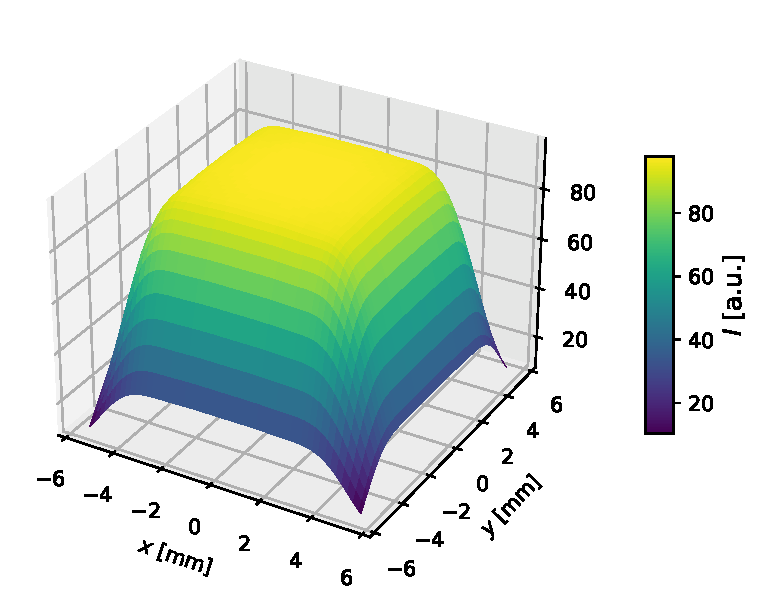
\includegraphics[width=\textwidth]{simplified-I-scattering-3D-plot-4.321}
		\caption{Scattering integrated over entire sample and normalized.}
		\label{fig:simplified-scattering-3D:b}
	\end{subfigure}
	\caption{An illustration of a simple scattering model assuming a very thin sample and single scattering of a square beam with $R=200\unit{\nano\meter}$, $\lambda_0 = 4.321$Å and $L_s = 1.8\unit\meter$. Beam divergence is neglected and a uniform profile is assumed. Figure \ref{fig:simplified-scattering-3D:a} shows the intensity contribution of a single point $(s_x,s_y) = (0,0)$ projected onto the detector. Figure \ref{fig:simplified-scattering-3D:b} shows the normalized result of integrating over the full $10\times10\unit{\milli\meter}$ sample, giving an indication of how much of the scattered fraction of neutrons is detected and which part of the detector can be used to reliably compute $G_\text{exp}$ without resorting to Monte Carlo methods.}
	\label{fig:simplified-scattering-3D}
\end{figure}
\begin{figure}[htbp]
	\centering
	\begin{subfigure}[b]{0.49\textwidth}
		\centering
		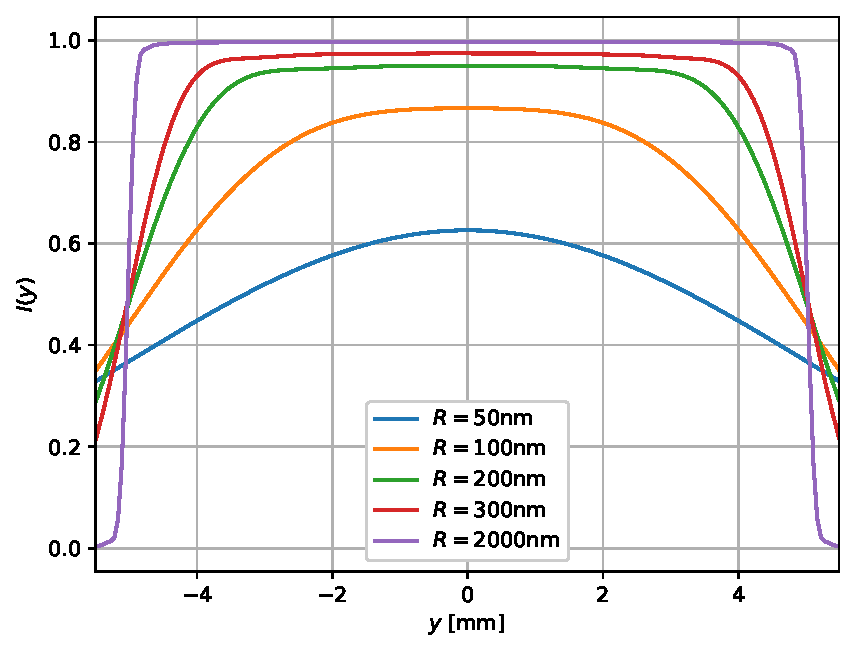
\includegraphics[width=\textwidth]{simplified-I-scattering-4.321}
		\caption{Estimated detected scattering fraction for $\lambda_0 = 4.321$Å}
		\label{fig:simplified-scattering-4.321}
	\end{subfigure}
	\hfill
	\begin{subfigure}[b]{0.49\textwidth}
		\centering
		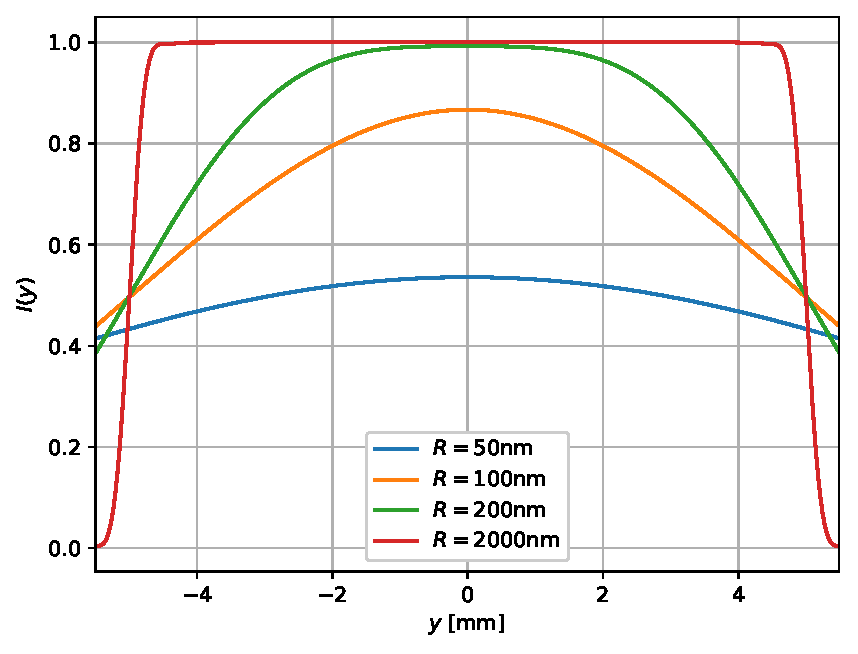
\includegraphics[width=\textwidth]{simplified-I-scattering-8.0}
		\caption{Estimated detected scattering fraction for $\lambda_0 = 8$Å}
		\label{fig:simplified-scattering-8}
	\end{subfigure}
	\caption{A comparison of the estimated fraction of scattered neutrons that is detected at each point on the detector with $L_s = 1.8\unit\meter$ for $\lambda_0 = 4.321$Å and $\lambda_0 = 8$Å and different radii $R$. Curves are calculated by first computing a 2D intensity pattern as illustrated in Figure \ref{fig:simplified-scattering-3D:b}, after which the pattern is integrated over $x$ and normalized.} 
	\label{fig:simplified-scattering}
\end{figure}
\subsubsection{Non-randomized single-scattering model}
A very thin, dilute sample of solid spheres has $d\sigma/d\Omega \propto P(Q)$ at each point in the sample $(s_x, s_y)$, neglecting effects like multiple scattering. The form factor $P(Q)$ of a solid sphere is given by Equation \eqref{eq:sample-form-factor}. Assuming a uniform square non-divergent beam where each neutrons scatters exactly once of the sample over an area of $10\times10\unit{\milli\meter}$, the corresponding detector intensity shape can be estimated by considering each point in the sample a source of scattering with intensity proportional to $P(Q)$, which can be translated to a point $(x,y)$ on the detector using trigonometry. The corresponding detector intensity shapes are found by integrating the scattering of many such points sources, a process shown in Figure \ref{fig:simplified-scattering-3D}. 


The intensity was integrated over the $x$-axis to give a single value for each point $y$, which is also what happens at a real linear 1D detector as considered in this work. Such integrated intensity profiles for different wavelengths and radii are shown in Figure \ref{fig:simplified-scattering}. It can be seen that the respective estimated limits of $100 \unit{\nano\meter}$ and $200 \unit{\nano\meter}$ describe the simplified scattering behaviour quite well, with these particle radii being approximately the limit where the middle of the detector picks up almost full intensity uniformly for a certain central width. Integrating these curves could provide another sample-dependent correction factor to complement the estimate given in Section \ref{c4.3} but Figure \ref{fig:simplified-scattering} also gives an idea at which radii error in $G_\text{exp}(\delta)$ becomes significant. This is an effect which can be corrected for \cite{kusmin2017}. It should be noted that Figure \ref{fig:simplified-scattering} only models the intensity of scattered neutrons and ignores multiple scattering. The scattering power $\tau = \sigma t$ of the sample as well as factors like beam divergence and uniformity will shape the true intensity shapes and $Q$-range of scattered neutrons.  Monte Carlo methods are more suitable for such more accurate calculations and this is the subject of Chapter \ref{c6:monte-carlo}.


\subsection{Design evaluation}
In this chapter, a wide range of effects limiting the $\delta$-range of designs have been discussed and computed for the design variants listed in Table \ref{tab:design-variants} with their various precession devices and $\lambda_0$-monochromator pairings. An optimistic order of magnitude estimate of intensity was made giving $10^5 \unit{\centi\meter^{-2}\sec^{-1}}$ and $10^6 \unit{\centi\meter^{-2}\sec^{-1}}$ for $\lambda_0 = 4.321$Å and $\lambda_0 = 8$Å respectively, the difference being due to the idealized VS monochromator passing through a broader spectrum. The various upper and lower $\delta$-limits imposed by the detector, precession devices and $\lambda$-spectrum width $\sigma$ were computed and are given in Table \ref{tab:designs-delta-constraints}, resulting in the final $\delta$-ranges as given in Table \ref{tab:designs-final-ranges}. It was also shown that for the given acceptance angle $\theta_a \approx h_d / (2L_s) = 3\unit{\milli\radian}$ at (approximately) maximal sample distance $L_s = 1.8\unit\meter$, and given these values of $\lambda_0$, it might prove to be difficult to access $\delta\propto 10\unit{\nano\meter}$. It would help to decrease $L_s$, increasing $\theta_a$ at the cost of slightly increasing the small-angle error as discussed in Section \ref{c3.5}. Simply decreasing $L_s$ would scale $\delta_{min}, \delta_{max}$ proportionately however, which in almost all cases would not improve the ability of instruments to measure the full target range of $10 \unit{\nano\meter}$ to $5000 \unit{\nano\meter}$ at a single sample to detector distance $L_s$ considering Table \ref{tab:designs-final-ranges}. Increasing $h_d$ would also increase $\theta_a$ without scaling down the $\delta$ range but this would potentially require a new detector. Such optimizations with more free parameters like distances $L_s, L_1, L_2$ are the subject of the next chapter. As was to be expected since $\delta \propto \lambda_0^2$, the designs at $\lambda_0 = 8$Å have higher maximum $\delta$ as well as having a smaller $Q_{max}$. As far as the precession devices are concerned, the great range in terms of $\alpha$ seems to make foil flippers and Wollaston prisms interesting options for an eventual realization. The range of the two instruments using isosceles triangles appears to be too limited to be practical in an instrument which requires a high $\delta_{max}/\delta_{min}$. Although the designs using foil flippers appear to perform the best in the sense of the limits given in Table \ref{tab:designs-final-ranges}, it should be noted that the $\lambda$-dependence \cite{kraan2003} of the foils was not considered here.

\newpage
\section{Constrained optimization of instrument parameters}
\label{c5:optimization}
As was illustrated in the previous chapters, the practical performance of a SEMSANS instrument in terms of $\delta$-range and intensity is a function of all of its parameters and components, making the design of instruments optimizing one or both of these design criteria a challenge. Although the analysis in Chapter \ref{c4:constraints} of the design variants listed in Table \ref{tab:design-variants} gives a first understanding of what is possible when designing an instrument at a cold source using different precession device choices and monochromator-$\lambda_0$ pairings, these designs are not optimized and are derivative of a simple previously simulated design \cite{bouwman2021b} using foil flippers and a thermal neutron source. In this chapter, the problem of designing an instrument is approached as a constrained optimization problem within the framework presented in Chapter \ref{c4:constraints}, focussing in particular on optimizing the accessible $\delta$-range. The goal is to provide an understanding of what is possible using different precession devices and monochromators when optimizing the parameters $\lambda_0, L_1, L_2, L_s$, with each parameter being appropriately bounded to ensure that $\lambda_0$ is compatible with the monochromator, $L_s$ allows a small-angle approximation together with detector height $h_d$ etc. 
To optimize an instrument computationally, an objective function needs to be formulated. Before this is done, some additional constraints are introduced which complete a formal description of the design constraints.
% TODO: change  precession devices and monochromators to 'precession devices, monochromators and detectors' if I do find time for h_d variation
%Two detector models will be considered: the first is the $11\times 11\unit{\milli\meter}$ detector with height $h_d = 11\unit{\milli\meter}$ and pixel size $p = 11\unit{\micro\meter}$ introduced in Section \ref{c3.4} and considered in the calculations presented in Chapter \ref{c4:constraints} as well as the simulations of Chapter \ref{c6:monte-carlo}; the second is a $40\times 40\unit{\milli\meter}$ detector with $h_d = 40\unit{\milli\meter}$ and the same pixel size $p = 11\unit{\micro\meter}$.


% TODO: FINISH THIS CHAPTER, ADDING OPTIMAL INSTRUMENT DESIGNS AND PERFORMANCE.
%The problem of designing an instrument suitable for a specific length range like $10 \unit{\nano\meter}$ to $5 \unit{\micro\meter}$ subject to the various constraints indicated in the previous chapter can be aptly described as a constrained optimization problem. This does require a formulation of an objective function to maximize and generally speaking this is easier said than done if all factors including instrument cost, intensity etc. are to be taken into account in addition to the $\delta$-range. In this section, the function that is maximized only depends on the $\delta$-range and consequently it should be understood as a speculative exploration of the instrument parameter-space rather than a final optimization of instruments to realize. At best, the presented optimal instruments represent the best one can do in terms of $\delta$-range in the framework of parameters and constraints considered in this research.

\subsection{Additional constraints for optimization}
\label{c5.1}
Although in an experimental setting this is obvious, the physical dimensions of in particular the precession components also play a role as well as the length of the total assembly. These restrictions complete the instrument description and make it possible to optimize instrument configurations computationally. If $L_1, L_2$ are considered to be the centre positions of the precession devices with depths $d_1, d_2$, the following condition limits $L_1$
$$L_1 \geq L_2 + \frac{d_1 + d_2}{2}$$
Similarly, the distance from sample to detector $L_s$ is bounded at least by
$$L_2 \geq L_s + \frac{d_2}{2}$$
This scheme could be further extended by considering the dimensions of the analyser, sample holder, monochromator etc. Additionally, $L_1$  will be bounded by in any case the length of the experiment hall the instrument is constructed in as well as by other factors. For simplicity, all precession devices are considered to have depth $d_1 = d_2 = 0.3\unit\meter$ as indicated in Chapter \ref{c3}. 
% and $L_s = 1.33\unit{\meter}$ for $h_d = 40\unit{\milli\meter}$.

%Although the modulation mechanism of SEMSANS appears to complicate this, it appears that the error 
% TODO: add spicy discussion in which I basically say: look, the error in the relation between phi_t and Q only becomes comparatively large for high delta, which corresponds to small Q making the error quite small again. So there is the crosswise effect which appears to make perhaps greater angles accessible across the board!

\subsection{Two possible $\delta$-range objective functions}
\label{c5.2}
Given the $\delta$ constraints formulated in Chapter \ref{c4:constraints} let $(\delta_{i, min},\delta_{i, max})$ be the final $\delta$ interval subject to these constraints and let $(\delta_{t, min},\delta_{t, max})$ be a target interval. If these overlap, let the overlap interval be given by $(\delta_{o, min},\delta_{o, max})$. A first objective function $g_1$ to maximize is ratio of the length of the overlap and the length of the target interval
$$g_1 = \begin{cases}
	\frac{\delta_{o, max}-\delta_{o, min}}{\delta_{t, max} - \delta_{t, min}},\text{ if $\delta$-ranges overlap}\\
	0,\text{ else}
\end{cases}$$
A potential problem with this objective function is that it does not take into consideration that the instrument should perform well across different length ranges and is biased towards the higher $\delta$ values in optimal designs. An intuitive way to optimize for coverage of different length ranges is achieved by looking at these on a logarithmic scale and considering the overlap there, which can be expressed using a second objective function $g_2$ as follows 
$$g_2 = \begin{cases}
	\frac{\ln(\delta_{o, max}/\delta_{o, min})}{\ln(\delta_{t, max}/\delta_{t, min})},\text{ if $\delta$-ranges overlap}\\
	0,\text{ else}
\end{cases}$$
%$g_1, g_2$ are two functions that can be optimized computationally to design instruments that best match a given target range like $10 \unit{\nano\meter}$ to $5 \unit{\micro\meter}$ or another preferred range. 

\subsection{Optimization scheme}
\label{c5.3}
Similar to in the previous chapter, all different pairings of precession devices and monochromators are considered. However, $\lambda_0, L_1, L_2, L_s$ are now free parameters with $\lambda_0$ being bounded by the approximate $\lambda$-band of the respective monochromator within the cold source spectrum, taken to be $3.0 - 4.4$Å and $8.0 - 12.0$Å for PG and VS respectively, and lengths bounded by the constraints given above. 
The instruments are optimized for target range $10 \unit{\nano\meter}$ to $5 \unit{\micro\meter}$ using objective function $g_2$, which prioritizes spanning all orders of magnitude of $\delta$ of the range. $L_1$ is limited to $5 \unit\meter$ to ensure a reasonable intensity for all designs. 

The used optimization routine is essentially a constrained random-search of the parameter space, generating $100000$ valid options for each combination of precession device and monochromator, choosing the generated combination of parameters which maximizes $g_2$. This is done by first generating a set of parameters each within their individual ranges and post-processing this to a parameter set which satisfies all constraints such as $L_1>L_2$ etc. by for instance swapping $L_1, L_2$ if $L_1 < L_2$. Naturally, the generated combination of parameters will not strictly be the (global) optimum and a certain level of noise in solution generation is expected. More proper methods like simulated annealing or gradient descent could be used to achieve more accurate optimal solutions with less noise but this is beyond the scope of this work.


% TODO: Switch to simulated annealing OR gradient descent for COOL OPTIMIZATION VIBES
% TODO: Add list of constraints somewhere to improve reproducibility?

\subsection{Optimized instruments}
The optimized instruments and their parameters are given in Table \ref{tab:optimized-designs}, their labels indicating the combination of monochromator and precession device of the instrument, which the parameters are optimized for in the sense of maximizing $g_2$. Their $\delta$-range and $Q_{max}$ is given in Table \ref{tab:optimized-designs-performance}, with $\delta_{min}, \delta_{max}$ being derived from Table \ref{tab:optimized-designs-delta-constraints} like in Section \ref{c4.2}.

\begin{table}[h!]
	\centering
	\begin{tabular}{c | c c c c c}
		\toprule
		Label & $\lambda_0$(Å) & $\Delta\lambda$(Å) & $L_1$($\unit{\meter}$) & $L_2$($\unit{\meter}$) & $L_s$($\unit{\meter}$) \\
		\midrule
		FOIL PG & 3.11 & 0.031 & 4.836 & 2.521 & 2.361 \\
		WSP PG & 4.4 & 0.044 & 4.827 & 0.518 & 0.358 \\
		ISO PG & 4.4 & 0.044 & 4.742 & 0.521 & 0.361 \\
		FOIL VS & 10.07 & 1.007 & 3.19 & 1.599 & 1.124 \\
		WSP VS & 8.86 & 0.886 & 4.764 & 1.438 & 1.278 \\
		ISO VS & 12.0 & 1.2 & 4.838 & 0.79 & 0.63 \\
		\bottomrule
	\end{tabular}
	\caption{Optimized design parameters for each combination of precession device option and monochromator. }
	\label{tab:optimized-designs}
\end{table}
Comparing the $\delta$-ranges in Table \ref{tab:optimized-designs-performance} with those of the unoptimized designs in Table \ref{tab:designs-final-ranges}, a first obvious difference is that far lower $\delta_{min}$ values are accessible to the optimized instruments. This comes at the cost of $\delta_{max}$ however with the new instruments optimized for $g_2$ in every case having a lower $\delta_{max}$. Comparing Table \ref{tab:optimized-designs-delta-constraints} to \ref{tab:designs-delta-constraints} shows that in both cases $\delta_{min,s}$ is the limiting factor, meaning that with $L_s$ and other parameters being optimized as far as possible, the detector height $h_d$ appears to restrict both the original and the optimized designs. The trend that in the upper $\delta$-range instruments with a PG monochromator and smaller $\lambda_0$ are more limited by their precession devices ($\delta_{max,d}$) and instruments with a VS monochromator and larger $\lambda_0$ more by the modulation envelope narrowing ($\delta_{max,e}$) also remains, as can be seen in Table \ref{tab:optimized-designs-delta-constraints}.


 Another difference is in $\theta_a$, taken to be approximately $\arctan(h_d/(2L_s))$. The optimized designs WSP PG and ISO PG have $\theta_a \approx 15\unit{\milli\radian}$ which is the used limit in optimization (see Section \ref{c3.5}). This means on one hand that if greater $\theta_a$ is possible, these instruments could probably be optimized further. On the other hand, if $15\unit{\milli\radian}$ is not feasible and the true limit is closer to $10\unit{\milli\radian}$ or $5\unit{\milli\radian}$, these designs cannot be realized and should be recomputed using a more appropriate limit. 

\begin{table}[h!]
	\centering
	\begin{tabular}{c|cc|ccc}
		\toprule
		Label & $\delta_{\text{min,s}}$ (nm) & $\delta_{\text{min,d}}$ (nm) & $\delta_{\text{max,s}}$ (nm) & $\delta_{\text{max,e}}$ (nm) & $\delta_{\text{max,d}}$ (nm) \\
		\midrule
		FOIL PG & 66.67 & \textbf{66.73} & 6674.06 & 32363.43 & \textbf{3478.05} \\
		WSP PG & \textbf{14.29} & 8.48 & 1430.77 & 6937.98 & \textbf{572.85} \\
		ISO PG & \textbf{14.45} & 8.34 & 1446.42 & 7013.89 & \textbf{137.55} \\
		FOIL VS & \textbf{102.89} & 100.87 & 10298.88 & \textbf{4994.07} & 5055.08 \\
		WSP VS & \textbf{103.0} & 34.23 & 10310.73 & \textbf{4999.81} & 6509.71 \\
		ISO VS & \textbf{68.69} & 68.5 & 6875.64 & 3334.09 & \textbf{1677.05} \\
		\bottomrule
	\end{tabular}
	\caption{Calculated $\delta$ constraints for optimized designs with the constraints limiting the final $\delta$-range listed in Table \ref{tab:optimized-designs-performance} marked in bold for each design.}
	\label{tab:optimized-designs-delta-constraints}
\end{table}

\begin{table}[h!]
	\centering
	\begin{tabular}{c | c c c c}
		\toprule
		Label & $Q_{\text{max}}$ ($\text{\AA}^{-1}$) & $\theta_a$ ($\unit{\milli\radian}$) & $\delta_{min}$ (nm) & $\delta_{max}$ (nm) \\
		\midrule
		FOIL PG & 0.00471 & 2.33 & 66.73 & 3478.05 \\
		WSP PG & 0.02198 & 15.375 & 14.29 & 572.85 \\
		ISO PG & 0.02174 & 15.217 & 14.45 & 137.55 \\
		FOIL VS & 0.00305 & 4.894 & 102.89 & 4994.07 \\
		WSP VS & 0.00305 & 4.303 & 103.0 & 4999.81 \\
		ISO VS & 0.00457 & 8.734 & 68.69 & 1677.05 \\
		\bottomrule
	\end{tabular}
	\caption{Key characteristics of optimized designs, with $\delta_{min}, \delta_{max}$ being computed using the constraints listed in Table \ref{tab:optimized-designs-delta-constraints}}
	\label{tab:optimized-designs-performance}
\end{table}

In conclusion, combining the constraint framework introduced in Chapter \ref{c4:constraints} with the method of numerical optimization has made it possible to identify the detector height $h_d$ (and the corresponding beam height, see Sections \ref{c3.2}, \ref{c3.4}) as a limitation for all SEMSANS instruments of the type described in Chapter \ref{c3} with length constraint $L_1 \leq 5 \unit\meter$. Increasing the beam height and detector height from $h_d = 11\unit{\milli\meter}$ to perhaps $h_d = 40\unit{\milli\meter}$ could be a first step towards realizing an instrument with $\delta$-range $10 \unit{\nano\meter}$ to $5 \unit{\micro\meter}$. An alternative would be to design a more powerful type of precession device.

%\subsection{Optimal designs for a larger detector height $h_d$}
%To complete the discussion

% TODO: find time to actually, properly talk about optimization results with bigger h_d without just rambling and stuff.

% The resulting optimal instrument parametrizations confirm patterns already visible in the previous chapter. For instance, isosceles triangles seem to be a very bad pairing with a PG monochromator. It can also be seen that instruments with PG monochromators are generally bounded on the upper end by field strength and those with velocity selectors by the narrowing of their envelope caused by wavelength spread. Similarly, almost all instruments are bounded by the condition that at least one period must be visible on the detector, with especially instruments at greater wavelengths $\lambda_0$ suffering from this limitation.  
% add further points that come up, maybe after writing a similar section for designs and their computed limitations



\newpage
\section{Monte Carlo simulations of designs using McStas}
\label{c6:monte-carlo}
In this chapter, Monte Carlo simulations of the instrument design variants using McStas \cite{willendrup2020} will be presented. The goal is to complement the analysis and constraints discussed in Chapter $\ref{c4:constraints}$ and provide an understanding of how instruments might behave in practice for a range of samples and how measurement data can be analysed. 

% after all the analysis and discussion of constraints/optimizing using these, introduce monte carlo simulations as a step closer to a practical instruments and a way to verify identified limitations and see them in play. This last aspect could be an interesting part of the discussion of simulation results as well, you can really point out narrowing modulation envelopes, modulation periods becoming too big for the detecto retcetera. 
% I expect some designs to not be able to measure specific samples at all or barely to the extent that showing them in a plot is a bit silly. 

\subsection{Method}
To test the ability of the various instruments to measure samples in the characteristic length range of $10 \unit{\nano\meter}$ to $5 \unit{\micro\meter}$ three samples of the type described in Section \ref{c2.4} are considered with radii $R = 50\unit{\nano\meter}, 300\unit{\nano\meter}, 2000\unit{\nano\meter}$. Although these could in principle all be simulated with other sample parameters like sample thickness $t$ the same, this would cause the scattering power $\tau$ as defined in Equation \eqref{eq:sample-tau} to vary greatly and cause it to go too far out of the range of $0.1$ and $0.8$ that is typically considered to be optimal in terms of signal-to-noise ratio \cite{bouwman2021b}\cite{heijkamp2011}. For this reason, $t$ is varied between $1 - 10\unit{\milli\meter}$ for different $\lambda_0, R$ pairings to optimize $\tau$. The remaining sample parameters take values $\phi = 0.015$, $\Delta\rho = 1.8\cdot 10^{10} \unit{\centi\meter}^{-2}$ and are the same in each case. The chosen $t$ values with the corresponding $\tau$ are shown in Table \ref{tab:sample-thickness}.


\begin{table}[h!]
	\centering
	\begin{tabular}{|c|c|c|c|}
		\hline
		$\lambda_0$ (Å)  & $R$ (nm)  & $t$ (mm)& $\tau$ \\
		\hline
		4.321 & 50 & 10 & 0.067\\
		4.321 & 300 & 10 & 0.4022 \\
		4.321 & 2000 & 1 & 0.2681 \\
		8 & 50 & 10 & 0.2298 \\
		8 & 300 & 5 & 0.6893 \\
		8 & 2000 & 1 & 0.9191 \\
		\hline
	\end{tabular}
	\caption{Combinations of $\lambda_0$ and sample radius $R$ with a sample thickness $t$ chosen to keep $\tau$ approximately within the optimal range of $0.1$ and $0.8$.}
	\label{tab:sample-thickness}
\end{table}
\subsubsection{Simulated measurement procedure}
For each instrument as described in Table \ref{tab:design-variants}, measurements on the three samples with radii and thicknesses as given in Table \ref{tab:sample-thickness} were simulated. Additionally, an empty measurement was done for each instrument to establish a baseline. 

To perform a measurement, a range of $B$-field strength values is simulated with the analyser in the $+x$ and $-x$ settings. Although in principle the full range of $B$-values bounded by the focussing condition could be simulated, only $B$-values were considered that correspond to the respective instrument $\delta$-range as given in Table \ref{tab:designs-final-ranges} in Chapter \ref{c4:constraints}. The sample range was taken to be $\frac{R}{10} - 3R$ and the overlap between each instrument range and these sample ranges were computed. In each case there was overlap and 30 $B$-settings corresponding to the overlapping $\delta$-range were chosen. $B$-resolution limitations were not considered here but can in practice be expected to limit the number of practical measurements to fewer than 30 as well as introducing $\delta$ uncertainty, becoming especially relevant in the lower $\delta$ range. 

\subsubsection{Simulation setup}
To simulate the instruments, version 3.4 of the raytracing software package McStas \cite{willendrup2020} is used with OpenACC acceleration enabled. The simulations were performed on a desktop computer with an Intel Core i5-6600 quad-core 3.3 Ghz CPU and an Nvidia GeForce GTX 1060 GPU. Simulated instruments are all derivative of the previously simulated \texttt{SEMSANS\_Delft} instrument \cite{bouwman2021b}. The \texttt{Foil\_flipper\_magnet} component was used to simulate foil flippers like in \texttt{SEMSANS\_Delft} and idealized components for the Wollaston prism and isosceles triangle were derived from the existing \texttt{Pol\_triafield} component. Each $B$-field and analyser setting was simulated using $10^7$ neutrons when using foil flippers and $10^8$ when using prisms or triangles. This due to the large difference in simulation time. Simulation time for a single simulation of $10^6$ varied from well under $1\unit{\second}$ for the prisms and triangles to about $4\unit{\second}$ for the foil flippers, presumably due to the greater complexity of the corresponding McStas component. 
The \texttt{SANS\_spheres2} sample component is used to model the described sample. Although most of its parameters correspond directly to those listed above, two that deserve mention are \texttt{Qmind} and \texttt{Qmaxd} which define the simulated $Q$-range. As the sample $R$ values span almost two orders of magnitude, the corresponding $Q$ range is quite different for the three samples and proportional to $1/R$. This is accounted for by using \texttt{Qmind}$=0.1/R$, \texttt{Qmaxd}$=10/R$, matching the sample $Q$-range as discussed in Section \ref{c2.4}.

\subsubsection{Data analysis}
To estimate $P(\delta) = e^{G(\delta)  - \tau}$, two data analysis methods are used on the simulation data. The first is based on fitting an expected modulation pattern as done elsewhere \cite{bouwman2011}\cite{parnell2023}, the second considers the RMS of the modulation pattern. The advantage of the second method is that it is more robust and better suited for real measurement conditions where many factors such as beam characteristics shape the observed modulation profile. Both rely on computing a quantity called the polarization $Pol(y)$\footnote{The choice for $Pol(y)$ instead of the more conventional $P(y)$ is deliberate and to avoid further overloading of $P$, which is already used in $P(\delta)$ and form factor $P(Q)$.}, defined as 
$$Pol(y) = \frac{I_{up}(y) - I_{down}(y)}{I_{up}(y) + I_{down}(y)}$$
Here $I_{up}, I_{down}$ correspond to simulated measurements using the $\pm x$ analyser settings. Intuitively, this gives a normalized expression for the modulation amplitude, allowing for some variation in total measured intensity $I_{up}(y) + I_{down}(y)$ across the detector. The signal at the boundaries of the detector is still not useful due to effects such as discussed in Section \ref{c4.4} and depicted in Figure \ref{fig:simplified-scattering} and only the middle $6\unit{\milli\meter}$ is used when estimating $P(\delta)$ for this reason.

In the first method, a modulation pattern with a Gaussian envelope similar to Equation \eqref{eq:poly-base-modulation} is fitted with variable amplitude to $Pol(y)$. Because $Pol(y)$ is used, $I_0$ disappears from the expression and $Pol_{b,s}(y)$ can largely be described by just $Pol_{\text{gauss}}(y) = A_{b,s}E(y)\cos(2\pi\alpha\lambda_0y)$ with fitted amplitudes $A_{b,s}$. In practice, a small error term $\epsilon$ is included to compensate for a potential non-zero average. This gives the final fitting function with parameter $A_{b,s}$
\begin{equation}
	Pol_{\text{fit}}(y) = \epsilon+ A_{b,s}E(y)\cos(2\pi\alpha\lambda_0y) \label{eq:gauss-fit-function}
\end{equation}
The resulting amplitudes $A_b, A_s$ with and without a sample at a given $B$ or $\delta$ setting are then related to $P(\delta)$ via $P_{exp}(\delta) = A_s/A_b$. 

In the second method, the RMS of $Pol(y)$ is computed as $RMS_{b,s}$ and again $P_{exp}(\delta)$ is given by the ratio $P_{exp}(\delta) = RMS_s/RMS_b$. The correctness of this method can be seen from the fact that for a single sinusoidal modulation the RMS is linearly proportional to the modulation amplitude. 

%As discussed in Section \ref{c3.6}, this can be expected to result in an error proportional to the width of the $\lambda$-spectrum, as a range of $\delta$'s is effectively sampled, each having their own $G(\delta)$ and $\tau(\delta)$. And as discussed in Sections \ref{c3.4} and \ref{c4.4}, the limited $Q$-range of the detector will result in incomplete detection of scattering for samples with smaller radii like $R = 50 \unit{\nano\meter}$ and a greater $Q$-range, limiting the accuracy of $G_\text{exp}(\delta)$. For these reasons, the value of $P(\delta)$ computed is to be understood as an estimate.  
\subsection{Results}
The result of the described simulation and data analysis using both methods is shown in Figures \ref{fig:simulation-plot-gauss}, \ref{fig:simulation-plot-rms}, with each subfigure showing simulated measurements within the accessible $\delta$-ranges for each design together with computed $P_{exp}(\delta)$ and analytical $P(\delta)$. Additionally, Figure \ref{fig:simulation-raw-intensity} shows an example of how raw simulation data from a simulated measurement using WSP 8 is processed and fitted to $P_{exp}(\delta)$ in the two ways. The corresponding values are $P_{exp} = 0.52187 \pm 0.0002$ when using the Gauss method and $P_{exp} = 0.516 \pm 0.004$ when using the RMS. The analytical value is $P(\delta) = 0.501906$, which is incompatible with both estimates and their standard error. These values were computed from fitted amplitudes $A_b = 0.999905 \pm 8\cdot 10^{-6}$, $A_s = 0.5218 \pm 0.0002$ and RMS values $RMS_b = 0.9999226 \pm 4\cdot 10^{-7}$ and $RMS_s = 0.517 \pm 0.004$. In both cases, the uncertainty with a sample is much greater than without.
\begin{figure}[htbp]
	\centering
	\begin{subfigure}[b]{0.45\textwidth}
		\centering
		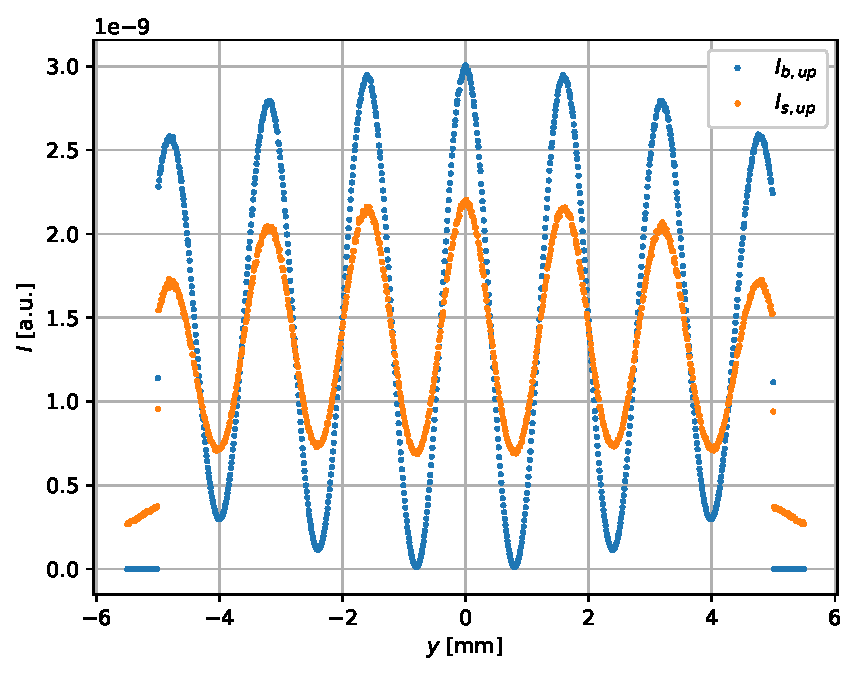
\includegraphics[width=\textwidth]{simulation-raw-intensity-up}
		\caption{$I_{b,up}$ and $I_{s,up}$ signals from }
		\label{fig:simulation-raw-intensity-up}
	\end{subfigure}
	\hfill
	\begin{subfigure}[b]{0.45\textwidth}
		\centering
		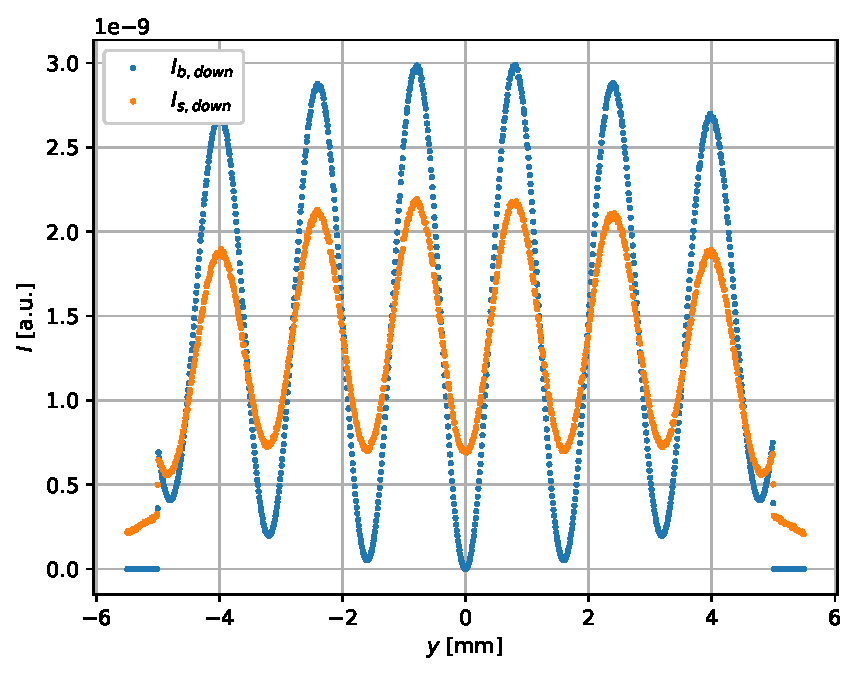
\includegraphics[width=\textwidth]{simulation-raw-intensity-down}
		\caption{$I_{b,down}$ and $I_{s,down}$}
		\label{fig:simulation-raw-intensity-down}
	\end{subfigure}
	\centering
	\begin{subfigure}[b]{0.45\textwidth}
		\centering
		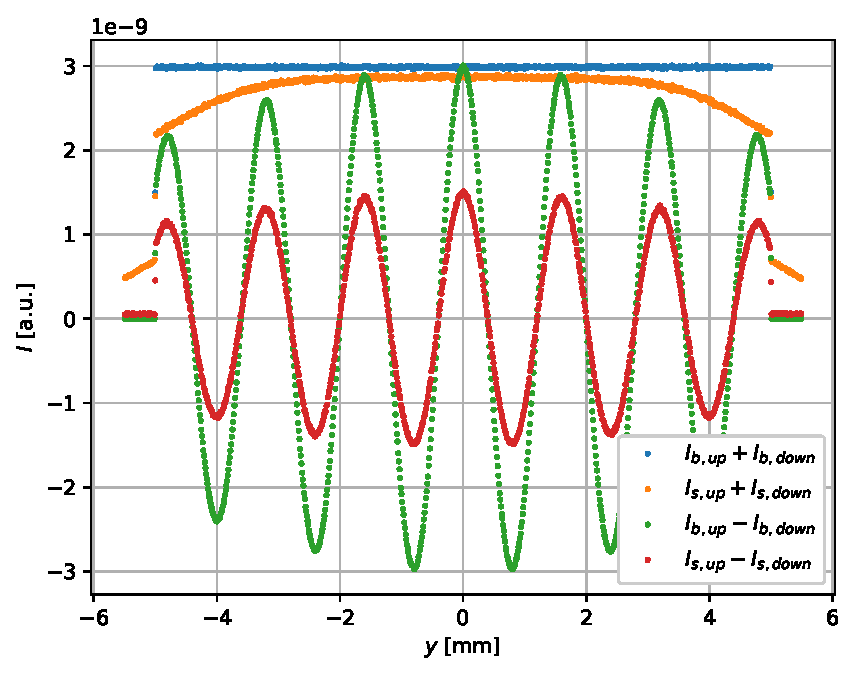
\includegraphics[width=\textwidth]{simulation-raw-intensity-differential}
		\caption{$I_{b,up} \pm I_{b,down}$ and $I_{s,up} \pm I_{s,down}$}
		\label{fig:simulation-raw-intensity-differential}
	\end{subfigure}
	\hfill
	\begin{subfigure}[b]{0.45\textwidth}
		\centering
		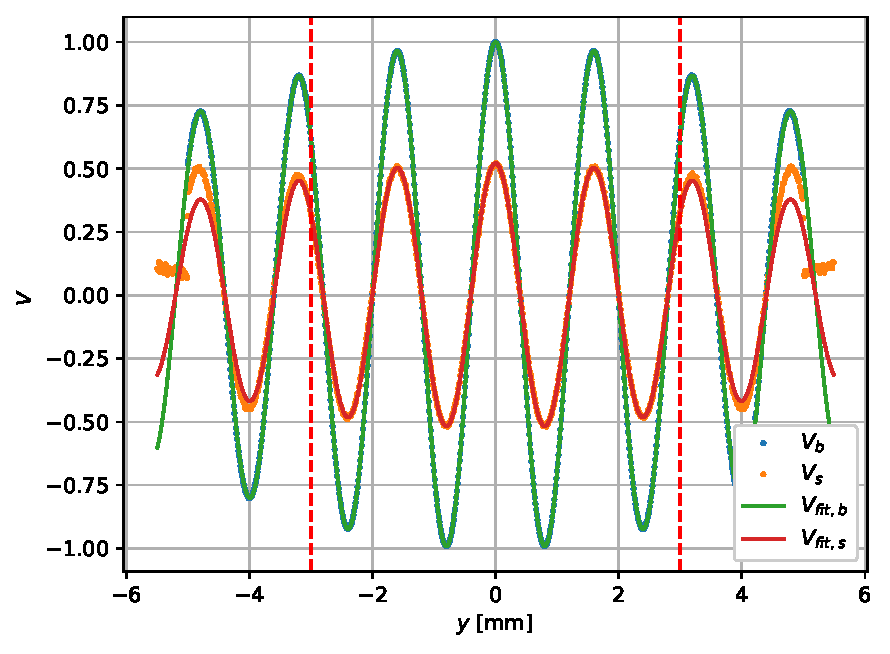
\includegraphics[width=\textwidth]{simulation-raw-intensity-pol}
		\caption{$Pol_b, Pol_s$ and}
		\label{fig:simulation-raw-intensity-pol}
	\end{subfigure}
	\caption{An illustration of the detector intensity patterns recorded during simulations and how they are processed to a fit. The data corresponds to a simulated measurement using WSP 8 of the $R = 300\unit{\nano\meter}$ sample with $B_1 = 5.4\unit{\milli\tesla}, B_2 = 10.8\unit{\milli\tesla}$, corresponding to $\delta = 900 \unit{\nano\meter}$. The fit values are shown in Figure \ref{fig:simulation-plot-gauss-WSP-8} and \ref{fig:simulation-plot-rms-WSP-8}. Figure \ref{fig:simulation-raw-intensity-up}, \ref{fig:simulation-raw-intensity-down} show the detector intensities overlaid with and without sample for both analyser settings (up and down). From these, signals are derived by adding and subtracting the up and down intensities. Finally, $Pol(y)$ is computed and from the $Pol(y)$ values in the middle $6\unit{\milli\meter}$ of the detector $P_{exp}(\delta)$ is computed by fitting modulation patterns with a Gaussian envelope or by computing the RMS.}
	\label{fig:simulation-raw-intensity}
\end{figure}

\begin{figure}[p]
	\centering
	\begin{subfigure}[b]{0.45\textwidth}
		\centering
		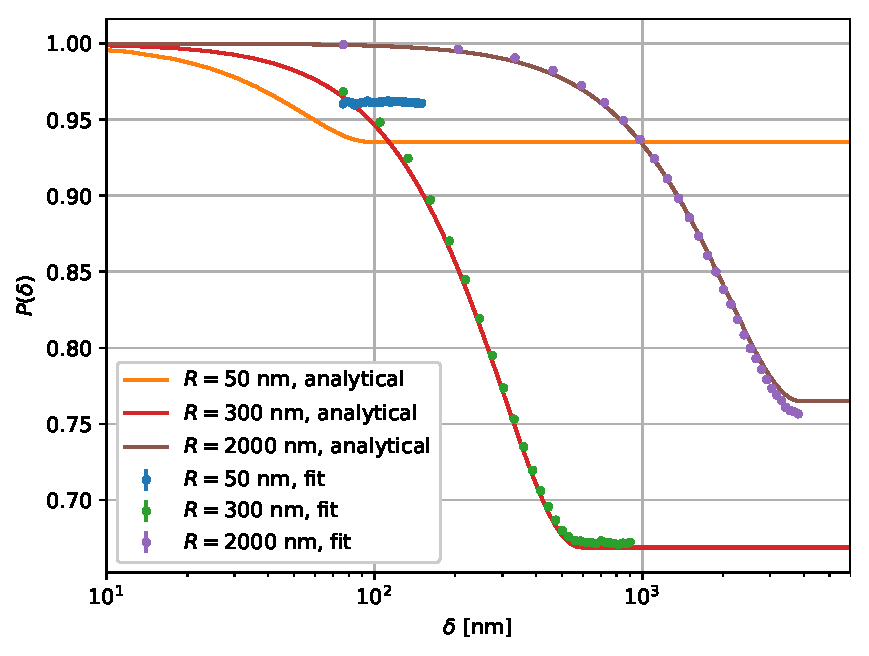
\includegraphics[width=\textwidth]{simulation-plot-gauss-FOIL-4.321}
		\caption{FOIL 4.321}
		\label{fig:simulation-plot-gauss-FOIL-4.321}
	\end{subfigure}
	\hfill
	\begin{subfigure}[b]{0.45\textwidth}
		\centering
		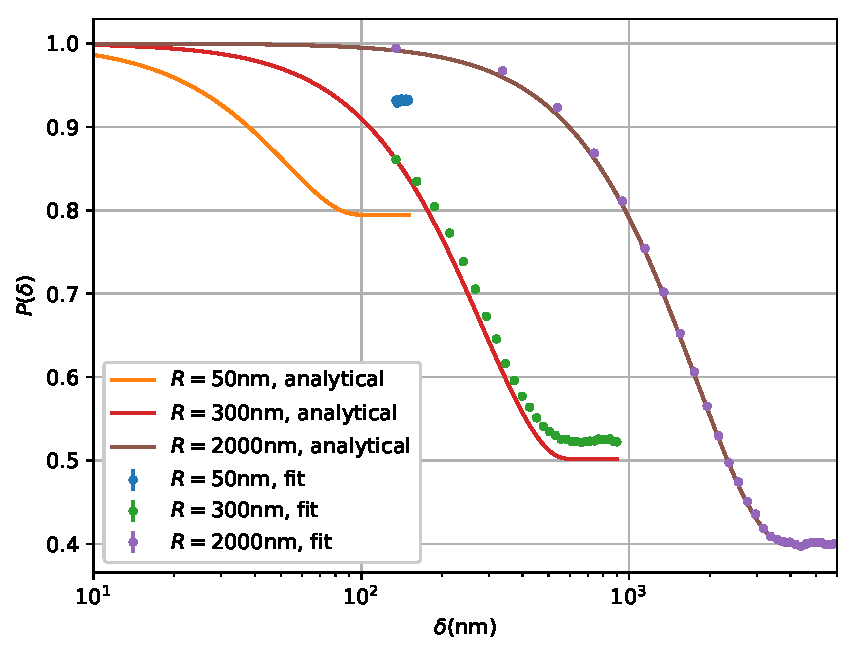
\includegraphics[width=\textwidth]{simulation-plot-gauss-FOIL-8}
		\caption{FOIL 8}
		\label{fig:simulation-plot-gauss-FOIL-8}
	\end{subfigure}
	\centering
	\begin{subfigure}[b]{0.45\textwidth}
		\centering
		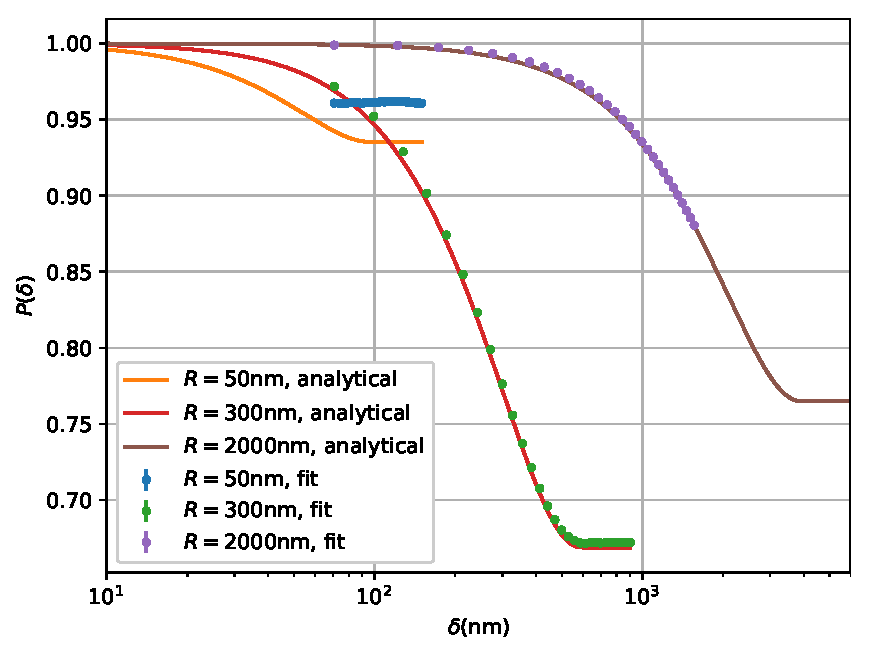
\includegraphics[width=\textwidth]{simulation-plot-gauss-WSP-4.321}
		\caption{WSP 4.321}
		\label{fig:simulation-plot-gauss-WSP-4.321}
	\end{subfigure}
	\hfill
	\begin{subfigure}[b]{0.45\textwidth}
		\centering
		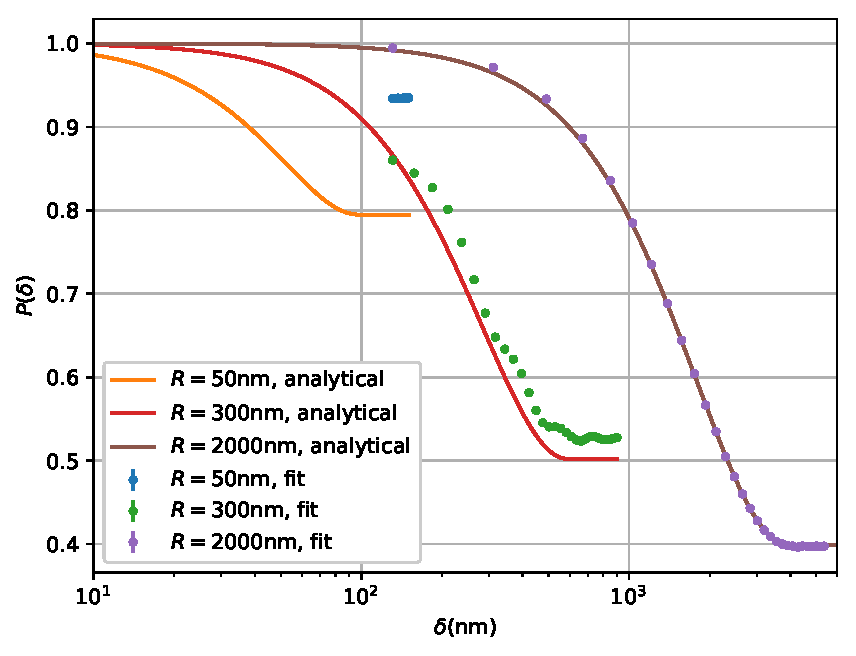
\includegraphics[width=\textwidth]{simulation-plot-gauss-WSP-8}
		\caption{WSP 8}
		\label{fig:simulation-plot-gauss-WSP-8}
	\end{subfigure}
	\centering
	\begin{subfigure}[b]{0.45\textwidth}
		\centering
		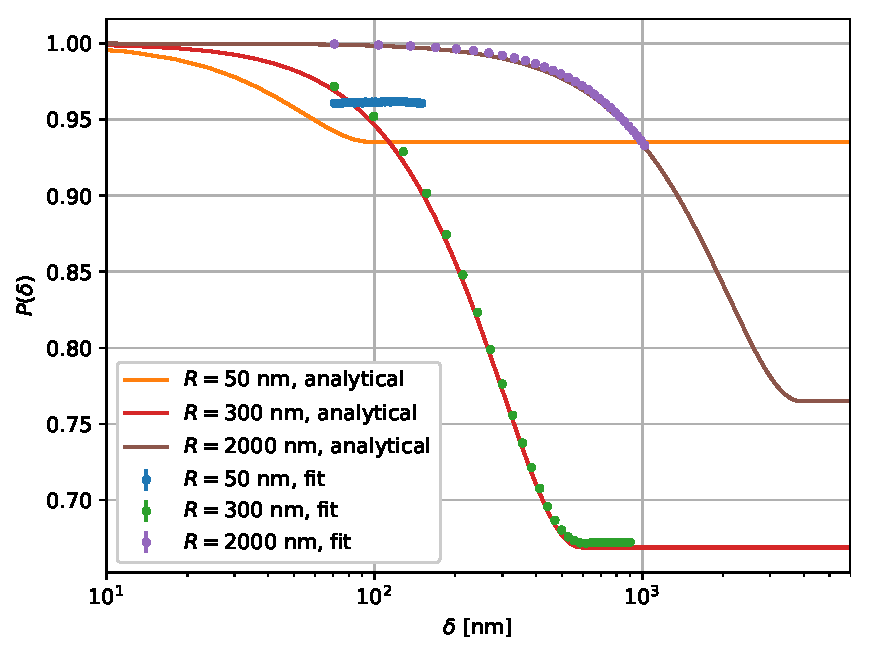
\includegraphics[width=\textwidth]{simulation-plot-gauss-ISO-4.321}
		\caption{ISO 4.321}
		\label{fig:simulation-plot-gauss-ISO-4.321}
	\end{subfigure}
	\hfill
	\begin{subfigure}[b]{0.45\textwidth}
		\centering
		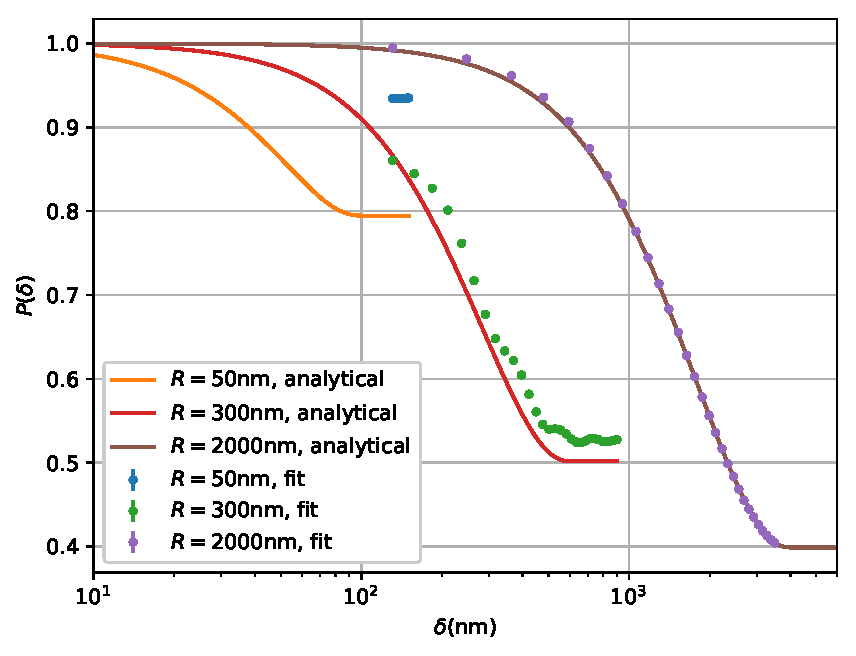
\includegraphics[width=\textwidth]{simulation-plot-gauss-ISO-8}
		\caption{ISO 8}
		\label{fig:simulation-plot-gauss-ISO-8}
	\end{subfigure}
	\caption{$P_{exp}(\delta)$ values derived from a fit of a Gaussian modulation envelope to detector intensity simulation data. Measurements using each of the six instruments were simulated using three samples as specified in Table \ref{tab:sample-thickness} together with the corresponding analytical $P(\delta)$. In most cases the error-bars are too small to be seen with exception of FOIL 4.321, FOIL 8, which were simulated using $10^7$ neutrons per measurement instead of $10^8$.}
	\label{fig:simulation-plot-gauss}
\end{figure}

\begin{figure}[p]
	\centering
	\begin{subfigure}[b]{0.45\textwidth}
		\centering
		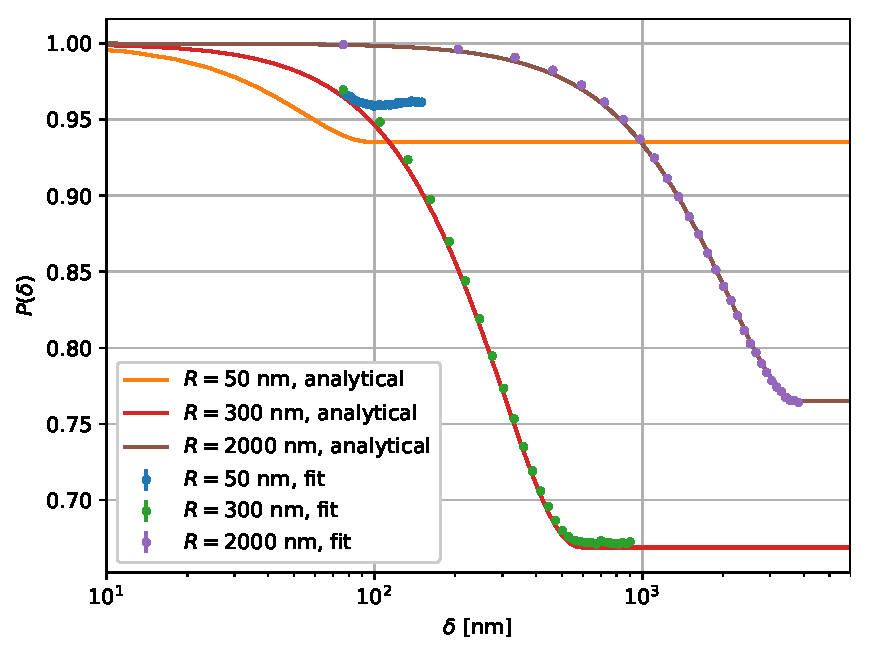
\includegraphics[width=\textwidth]{simulation-plot-rms-FOIL-4.321}
		\caption{FOIL 4.321}
		\label{fig:simulation-plot-rms-FOIL-4.321}
	\end{subfigure}
	\hfill
	\begin{subfigure}[b]{0.45\textwidth}
		\centering
		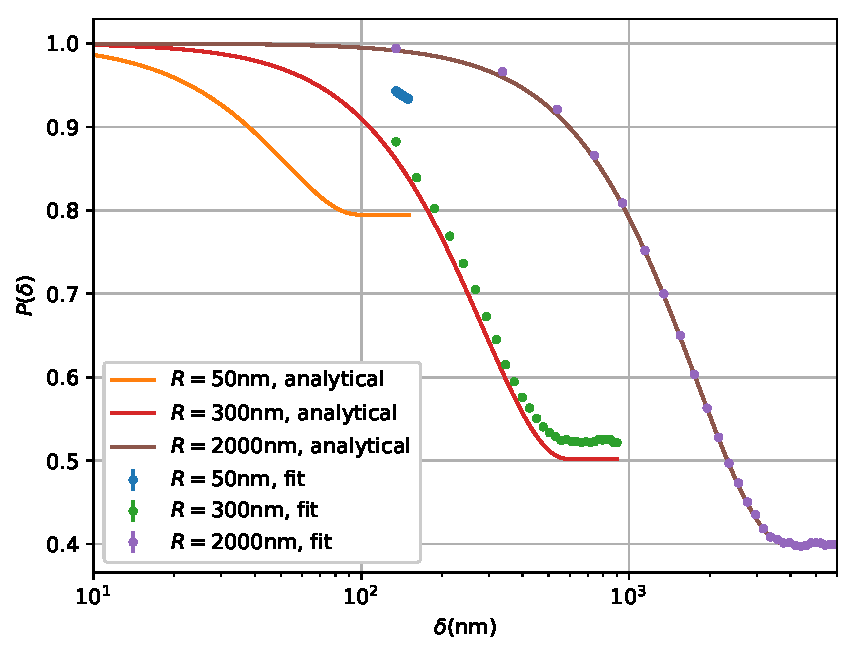
\includegraphics[width=\textwidth]{simulation-plot-rms-FOIL-8}
		\caption{FOIL 8}
		\label{fig:simulation-plot-rms-FOIL-8}
	\end{subfigure}
	\centering
	\begin{subfigure}[b]{0.45\textwidth}
		\centering
		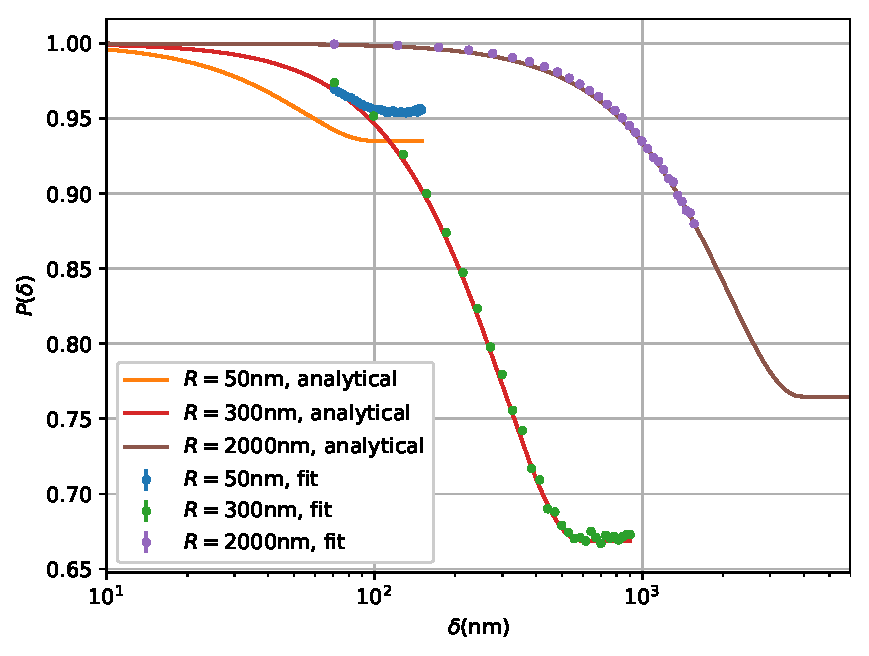
\includegraphics[width=\textwidth]{simulation-plot-rms-WSP-4.321}
		\caption{WSP 4.321}
		\label{fig:simulation-plot-rms-WSP-4.321}
	\end{subfigure}
	\hfill
	\begin{subfigure}[b]{0.45\textwidth}
		\centering
		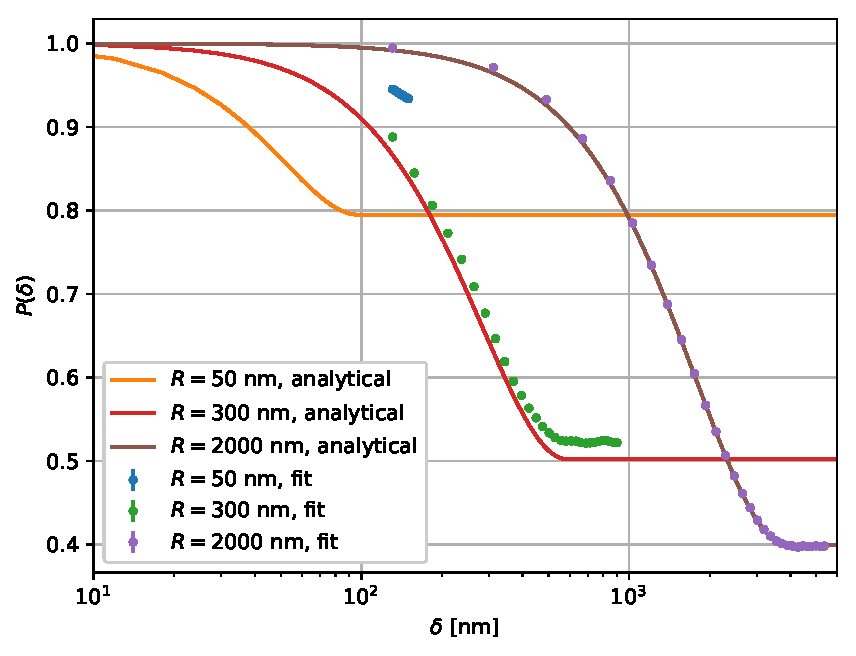
\includegraphics[width=\textwidth]{simulation-plot-rms-WSP-8}
		\caption{WSP 8}
		\label{fig:simulation-plot-rms-WSP-8}
	\end{subfigure}
	\centering
	\begin{subfigure}[b]{0.45\textwidth}
		\centering
		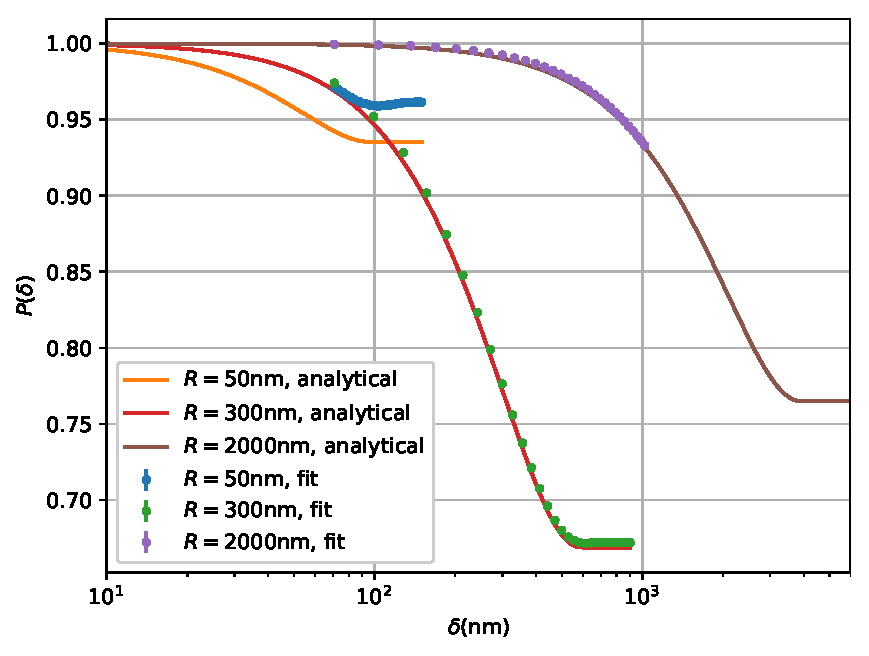
\includegraphics[width=\textwidth]{simulation-plot-rms-ISO-4.321}
		\caption{ISO 4.321}
		\label{fig:simulation-plot-rms-ISO-4.321}
	\end{subfigure}
	\hfill
	\begin{subfigure}[b]{0.45\textwidth}
		\centering
		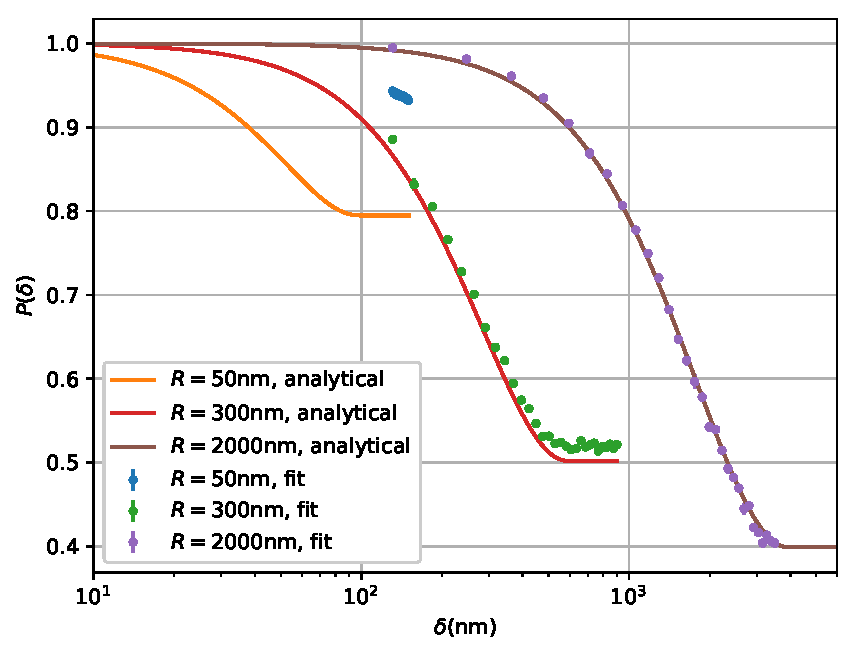
\includegraphics[width=\textwidth]{simulation-plot-rms-ISO-8}
		\caption{ISO 8}
		\label{fig:simulation-plot-rms-ISO-8}
	\end{subfigure}
	\caption{$P_{exp}(\delta)$ values derived using the RMS method together with analytical $P(\delta)$ curves for three different samples. The data is the same as shown in Figure \ref{fig:simulation-plot-gauss}.}
	\label{fig:simulation-plot-rms}
\end{figure}

\subsection{Discussion}
When comparing Figures \ref{fig:simulation-plot-gauss}, \ref{fig:simulation-plot-rms}, it appears that generally speaking both analysis methods give similar results. While the RMS method is more noise sensitive as can be seen from fits like Figure \ref{fig:simulation-plot-rms-FOIL-4.321} as compared to \ref{fig:simulation-plot-gauss-FOIL-4.321}, it seems to give more consistent results, giving a more reasonable fit of the $R=50\unit{\nano\meter}$ sample by appearing to capture some of the curvature of $P(\delta)$ in Figure \ref{fig:simulation-plot-rms-WSP-4.321}. Although corrections compensating for a too low detector $Q$-range \cite{kusmin2017} were not performed, it could be that the corrected analytical $P(\delta)$ curve for this sample looks somewhat like the $P_{exp}(\delta)$ fitted to data. Both methods also give a $P_{exp}(\delta)$ for $R = 300 \unit{\nano\meter}$ that is shifted upwards compared to the expected $P(\delta)$ for all instruments with $\lambda_0 = 8$Å, indicating that $P_{exp}(\delta)$ probably accurately describes the fitted $y$-range of $Pol(y)$ data but cannot simply be said to estimate $P(\delta)$. Fitting only the middle $2\unit{\milli\meter}$ instead of the middle $6\unit{\milli\meter}$ of the detector reduces this error somewhat but not entirely. This can perhaps be explained by the relatively high $\tau = 0.6893$ as listed in Table \ref{tab:sample-thickness}, causing a relatively higher degree of multiple scattering and a larger fraction of scattered neutrons to go undetected making $P_{exp}(\delta)$ a poor estimate of $P(\delta)$. Another reason could be the greater $\Delta\lambda$ of designs at $\lambda_0 = 8$Å, causing errors of the type discussed in Section \ref{c3.6} in addition to a greater spread scattering angles as $Q\propto 1/\lambda$, making the same $Q$ scatter into larger angles for higher $\lambda$, reducing the quality of estimate $P_{exp}(\delta)$ and the effective $Q$-range of the instrument.

This could mean that instruments with $\Delta\lambda/\lambda_0 = 0.1$ or similar like the three presented here with $\lambda_0 = 8$Å are more restricted for lower values of $\delta$ than predicted using the constraint model presented in Chapter \ref{c4:constraints} (which only considered $\Delta\lambda$ as having an effect on the modulation envelope), meaning that measuring wide $\delta$ ranges might be harder when using colder wavelengths available at a $T=20K$ using a velocity selector. 

% TODO add table illustrating different intensity

% None of the instruments were able to fully characterize the $R=50\unit{\nano\meter}$ sample, with the previously computed (hard) constraints listed limiting the $\delta$-range. 


%Although the instruments operating at $\lambda_0 = 4.321$Å were able to measure a somewhat wider range, all that can be said about these and those with $\lambda_0 = 8$Å is that they managed to estimate $P(\infty) = e^{-\tau}$ for this sample to differing degrees of accuracy. All instruments were able to measure the $R = 2000 \unit{\nano\meter}$ sample well within their given $\delta$ limitations, with all designs except WSP 4.321 and ISO 4.321 being able to measure up to $\delta \approx 2R$. Going by the analysis presented in Section \ref{c4.4}, it was expected that for $\lambda_0 = 4.321, 8$Å the approximate lower limit at which SEMSANS ceases to approximate $P(\delta)$ well is $100, 200\unit{\nano\meter}$ respectively. This appears to be reflected in the increasing error compared to the analytical expression for $R = 300\unit{\nano\meter}$ which has not been corrected for such an effect. The error is greater for $\lambda_0 = 8$Å which makes sense given what was discussed in Section \ref{c4.3}. This error can be reduced by fitting a smaller height than the centre $8\unit{\milli\meter}$, trading correctness of the estimate for increased uncertainty in $P(\delta)$, which can be understood by considering Figure \ref{fig:simplified-scattering} and the fraction of scattered neutrons that is 'missing' from each point on the detector. 

%\subsubsection{Comparison of analysis methods}
%When comparing Figures \ref{fig:simulation-plot-gauss}, \ref{fig:simulation-plot-rms}, it appears that generally speaking both analysis methods give similar results. While the RMS method is more noise sensitive as can be seen from fits like Figure \ref{fig:simulation-plot-rms-FOIL-4.321} as compared to \ref{fig:simulation-plot-gauss-FOIL-4.321}, it seems to give more consistent results, giving a more reasonable fit of the $R=50\unit{\nano\meter}$ sample by appearing to capture some of the curvature of $P(\delta)$. Although corrections compensating for a too low detector $Q$-range \cite{kusmin2017} were not performed, it could be that the corrected analytical $P(\delta)$ curve for this sample looks somewhat like what is fitted. 

% Did the simulations match the precomputed limits? Are the limits (to the extent that they are not absolute but rather somewhat chosen heuristically) good enough, too strict? Is it in practice possible to measure even at field strenghts outside of the range?

\newpage
\section{Conclusion and future work}
In this work, the possibility of realizing a SEMSANS instrument at the new cold source at the Hoger Onderwijs Reactor at the Reactor Institute in Delft was explored through a combination of mathematical analysis, constrained optimization and Monte Carlo simulations. After providing an overview of relevant theory and introducing a simplified instrument model, six combinations of three precession device options and two monochromator types with compatible wavelengths $\lambda_0$ were presented. These were analysed in detail and measurements of known samples were simulated using the raytracing software package McStas \cite{willendrup2020}. 

The goal was to explore possibilities for an instrument that could be used to measure processes in the range of $10 \unit{\nano\meter}$ to $5 \unit{\micro\meter}$. It was shown by optimizing all available free parameters that when considering a beam size and detector height of $10\unit{\milli\meter}$ in an instrument no more than about $5 \unit\meter$ in length, it is impossible to measure this full range keeping the distance from sample to detector $L_s$ constant. This might be possible however if a larger beam and detector is used or if more powerful precession devices become available as these were identified to be limiting factors both for an initial set of designs and optimized designs.

The effects of using a monochromator with a greater $\Delta\lambda/\lambda_0$ in terms of modulation patterns and scattered intensity were analysed in detail and it appears from simulation results that instruments selecting very cold neutrons (i.e. $\lambda_0 = 8$Å or above) using a velocity selector might be harder to realize than instruments using a more selective pyroletic graphite monochromator with  $\lambda_0 = 4.321$Å or so due to the greater spread in scattering angles when using a broader spectrum. 

\subsection{Future work}
The purpose of this work was to give a first understanding of what is possible in terms of designing SEMSANS instruments for the cold source. For this reason, a great number of factors were abstracted and the instrument designs analysed were in many ways idealized. For instance, the beam was considered to have a uniform profile with slight divergence which was often neglected and a $\lambda$-spectrum exactly described by a Maxwell-Boltzmann spectrum at $T=20\unit\kelvin$, with a Gaussian distribution of wavelengths being selected from it using an idealized monochromator. These and other simplifications leave a lot of work to be done in terms of more realistic analysis and simulations taking into consideration the true profile and spectrum of the cold source as well as how the source is in practice collimated. The same goes for simulating the physical precession devices, monochromators, polarizer and the analyzer. This would also make more accurate intensity estimates possible which is an important step before any potential realization of an instrument. Lastly, more detailed studies of tolerable acceptance angles in SEMSANS as well as the effect of broader $\lambda$-spectra on measurement ranges would make it possible to optimize designs further than was done in this work and make it easier to estimate what can practically be measured using a given design.

\newpage
\printbibliography

\appendix
\section{Limitations of SEMSANS theory at lower end of $\delta$ range}
\label{appendix-a}
In elastic scattering, the initial and final wave vectors $k_i$, $k_f$ are related through wave vector transfer $Q = |k_f - k_i| = k 2\sin\theta$ with $2\theta$ being the angle between $k_i, k_f$ and $|k_i| = |k_f| = k$ due to elasticity. In normal SEMSANS theory, the small-angle approximation must hold so that $Q_y = k2\theta$ or with $2\theta \approx \frac{y}{L_s}$, $Q_y = k\frac{y}{L_s}$. Using this approximation, it can be seen that $\phi_t = \delta Q_y$, which means that the modulation amplitude $A_s(\delta), A_b(\delta)$ with and without sample is related to $G(\delta)$
% $$G(\delta) = \frac{t}{k^2}\int_{Q_{x,min}}^{Q_{x,max}}\int_{Q_{y,min}}^{Q_{y,max}}\dfrac{d\sigma}{d\Omega}(Q)\cos(\delta Q_y)dQ_ydQ_x$$
by the formula
$$\frac{A_s(\delta)}{A_b(\delta)} = e^{G(\delta) - \tau}$$
It can be shown that the generally correct expression for $Q_y$ is 
$$Q_y = 2k\sin(\frac{\arctan\frac{y}{L_s}}{2})$$
%This can be simplified to the somewhat lengthy expression
%$$Q_y = 2k \frac{\frac{y}{L_s}}{\sqrt{2}\sqrt{\frac{y^2}{L_s^2} + 1 }\sqrt{\frac{1}{\sqrt{\frac{y^2}{L_s^2} + 1}}+1}}$$ 
Considering again small $\frac{y}{L_s}$, it can be derived using a Taylor expansion that in third-order approximation 
$$Q_y \approx  k(\frac{y}{L_s} - \frac{3y^3}{8L_s^3})$$
%So a more accurate relation between $\phi_t$ and $Q, \delta_y$ is given by $$\phi_t = \frac{\delta Q_y}{1 - \frac{3y^2}{8L_s^2}}$$ This appears to give an indication of up to which angles the SEMSANS theory gives a correct description of the amplitude decrease.
\end{document}
